%\right \right \right \right \right \right \right \right \right \right \right \right \right \right \right \right \right \right \right \right \right \right \right \right \right \right \right \right \right \right \right \right \right \right \right \right \right \right \right \right \right \right \right \right \right \right \right \right \right 	~~~~~~~~```% This is "sig-alternate.tex" V2.0 May 2012
% This file should be compiled with V2.5 of "sig-alternate.cls" May 2012
%
% This example file demonstrates the use of the 'sig-alternate.cls'
% V2.5 LaTeX2e document class file. It is for those submitting
% articles to ACM Conference Proceedings WHO DO NOT WISH TO
% STRICTLY ADHERE TO THE SIGS (PUBS-BOARD-ENDORSED) STYLE.
% The 'sig-alternate.cls' file will produce a similar-looking,
% albeit, 'tighter' paper resulting in, invariably, fewer pages.
%
% ----------------------------------------------------------------------------------------------------------------
% This .tex file (and associated .cls V2.5) produces:
%       1) The Permission Statement
%       2) The Conference (location) Info information
%       3) The Copyright Line with ACM data
%       4) NO page numbers
%
% as against the acm_proc_article-sp.cls file which
% DOES NOT produce 1) thru' 3) above.
%
% Using 'sig-alternate.cls' you have control, however, from within
% the source .tex file, over both the CopyrightYear
% (defaulted to 200X) and the ACM Copyright Data
% (defaulted to X-XXXXX-XX-X/XX/XX).
% e.g.
% \CopyrightYear{2007} will cause 2007 to appear in the copyright line.
% \crdata{0-12345-67-8/90/12} will cause 0-12345-67-8/90/12 to appear in the copyright line.
%
% ---------------------------------------------------------------------------------------------------------------
% This .tex source is an example which *does* use
% the .bib file (from which the .bbl file % is produced).
% REMEMBER HOWEVER: After having produced the .bbl file,
% and prior to final submission, you *NEED* to 'insert'
% your .bbl file into your source .tex file so as to provide
% ONE 'self-contained' source file.
%
% ================= IF YOU HAVE QUESTIONS =======================
% Questions regarding the SIGS styles, SIGS policies and
% procedures, Conferences etc. should be sent to
% Adrienne Griscti (griscti@acm.org)
%
% Technical questions _only_ to
% Gerald Murray (murray@hq.acm.org)
% ===============================================================
%
% For tracking purposes - this is V2.0 - May 2012

\documentclass{sig-alternate}
\usepackage[normalem]{ulem}
\usepackage{algpseudocode}
\usepackage{algorithm}
\usepackage{amsmath}
%\usepackage{url}
\usepackage{graphicx}
\usepackage{subfigure}

\usepackage{footnote}
\makesavenoteenv{tabular}
\makesavenoteenv{table}

\algrenewcommand{\algorithmicrequire}{\textbf{Input:}}
\algrenewcommand{\algorithmicensure}{\textbf{Output:}}
\renewcommand{\algorithmicforall}{\textbf{for each}}

\begin{document}
%
% --- Author Metadata here ---
\conferenceinfo{WOODSTOCK}{'97 El Paso, Texas USA}
%\CopyrightYear{2007} % Allows default copyright year (20XX) to be over-ridden - IF NEED BE.
%\crdata{0-12345-67-8/90/01}  % Allows default copyright data (0-89791-88-6/97/05) to be over-ridden - IF NEED BE.
% --- End of Author Metadata ---

\title{Identify failure-inducing combinations for multiple faults\titlenote{This work was supported by the National Natural Science Foundation of China (No. 61272079), the Research Fund for the Doctoral Program of Higher Education of China (No.20130091110032), the Science Fund for Creative Research Groups of the National Natural Science Foundation of China(No. 61321491), and the Major Program of National Natural Science Foundation of China (No. 91318301)}
}
%
% You need the command \numberofauthors to handle the 'placement
% and alignment' of the authors beneath the title.
%
% For aesthetic reasons, we recommend 'three authors at a time'
% i.e. three 'name/affiliation blocks' be placed beneath the title.
%
% NOTE: You are NOT restricted in how many 'rows' of
% "name/affiliations" may appear. We just ask that you restrict
% the number of 'columns' to three.
%
% Because of the available 'opening page real-estate'
% we ask you to refrain from putting more than six authors
% (two rows with three columns) beneath the article title.
% More than six makes the first-page appear very cluttered indeed.
%
% Use the \alignauthor commands to handle the names
% and affiliations for an 'aesthetic maximum' of six authors.
% Add names, affiliations, addresses for
% the seventh etc. author(s) as the argument for the
% \additionalauthors command.
% These 'additional authors' will be output/set for you
% without further effort on your part as the last section in
% the body of your article BEFORE References or any Appendices.

\numberofauthors{2} %  in this sample file, there are a *total*
% of EIGHT authors. SIX appear on the 'first-page' (for formatting
% reasons) and the remaining two appear in the \additionalauthors section.
%
\author{
% You can go ahead and credit any number of authors here,
% e.g. one 'row of three' or two rows (consisting of one row of three
% and a second row of one, two or three).
%
% The command \alignauthor (no curly braces needed) should
% precede each author name, affiliation/snail-mail address and
% e-mail address. Additionally, tag each line of
% affiliation/address with \affaddr, and tag the
% e-mail address with \email.
%
% 1st. author
\alignauthor
Xintao Niu\\
       \affaddr{State Key Laboratory for Novel Software Technology}\\
       \affaddr{Nanjing University}\\
       \affaddr{China, 210023}\\
       \email{niuxintao@smail.nju.edu.cn}
% 2nd. author
\alignauthor
Changhai Nie\\
       \affaddr{State Key Laboratory for Novel Software Technology}\\
       \affaddr{Nanjing University}\\
       \affaddr{China, 210023}\\
       \email{changhainie@nju.edu.cn}
% 3rd. author
}
% There's nothing stopping you putting the seventh, eighth, etc.
% author on the opening page (as the 'third row') but we ask,
% for aesthetic reasons that you place these 'additional authors'
% in the \additional authors block, viz.
% Just remember to make sure that the TOTAL number of authors
% is the number that will appear on the first page PLUS the
% number that will appear in the \additionalauthors section.
\maketitle
\begin{abstract}
Combinatorial testing(CT) is proven to be effective to reveal the potential failures caused by the interaction of the inputs or options of the system under test(SUT). A key problem in CT is to isolate the failure-inducing interactions of the related failure as it can facilitate the debugging effort by reducing the scope of code that needs to be inspected. Many algorithms has been proposed to identify the failure-inducing interactions, however, most of these studies either just consider the condition of one fault or ignore masking effects among multiple faults which can bias their identified results. In this paper, we analysed how the masking effect of multiple faults affect on the isolation of failure-inducing interactions. We further give a strategy of selecting test cases to alleviate this impact. Our approach first prune these test cases that may trigger masking effect and then generate no-masking-effect ones to test the interactions supposed to be tested in these pruned test cases. The test-case selecting process repeated until we get enough information to isolate the failure-inducing interactions. We conducted some empirical studies on several open-source software. The result of the studies shows that multiple faults as well as the masking effects do exist in real software and our approach can assist combinatorial-based failure-inducing identifying methods to get a better result when handling multiple faults in SUT.
\end{abstract}

% A category with the (minimum) three required fields
%\category{H.4}{Information Systems Applications}{Miscellaneous}
%A category including the fourth, optional field follows...
\category{D.2.5}{Software Engineering}{Testing and debugging}[Debugging aids,testing tools]

\terms{Reliability, Verification}

\keywords{Software Testing, Combinatorial Testing, Failure-inducing combinations, Masking effects} % NOT required for Proceedings

\section{Introduction}

With the increasing complexity and size of modern software, many factors, such as input parameters and configuration options, can influence the behaviour of the system under test(SUT). The unexpected faults caused by the interaction among these factors can make testing such software a big challenge if the interaction space is too large. One remedy for this problem is combinatorial testing, which systematically sample the interaction space and select a relatively small size of test cases that cover all the valid iterations with the number of factors involved in the interaction no more than a prior fixed integer, i.e., the \emph{strength} of the interaction.

Once failures are detected, it is desired to isolate the failure-inducing interactions in these failing test cases. This task is important in CT as it can facilitate the debugging effort by reducing the code scope that needed to inspected. Many algorithms has been proposed to identify the failure-inducing interactions in SUT, which include approaches such as building classification tree model \cite{yilmaz2006covering}, generating one test case one time \cite{nie2011minimal}, ranking suspicious interactions based on prior rules\cite{ghandehari2012identifying}, using graphic-based deduction \cite{martinez2008algorithms} and so on. These approaches can be partitioned into two categories \cite{colbourn2008locating}: \emph{adaptive}--tests cases are chosen based on the outcomes of the executions of prior tests \cite{nie2011minimal,ghandehari2012identifying,niu2013identifying,zhang2011characterizing,shakya2012isolating,wang2010adaptive,li2012improved}or \emph{nonadaptive}--test cases are chosen independent and can be executed parallel \cite{yilmaz2006covering,colbourn2008locating,martinez2008algorithms,martinez2009locating,fouche2009incremental}.

%jieLi and paritiion

While all these approaches can help developers to isolate the failure-inducing factors in failing test cases, in our recently studies on several open-source software, however, we found these approaches suffered from \emph{masking effects} of multiple faults in SUT. A masking effect \cite{dumlu2011feedback,yilmaz2013reducing} is an effect that some failures prevents test cases from normally checking combinations that are supposed to be tested. Take the Linux command-- \emph{Grep} for example, we noticed that there are two different faults reported in the bug tracker system. The first one \footnote{http://savannah.gnu.org/bugs/?29537}  claims that Grep incorrectly match unicode patterns with '\textbackslash<\textbackslash>', while the second one \footnote{http://savannah.gnu.org/bugs/?33080} claims a incompatibility between option '-c' and '-o'. When we put this two scenario into one test case only one fault information will be observed, which means another fault is masked by the observed one. This effect was firstly introduced by Dumllu and Ylimaz in \cite{dumlu2011feedback}, in which they found that the masking effects in CT can make traditional covering array failed detecting some combinations and they proposed a feedback-driven approach to work around them. Their recent work \cite{yilmaz2013reducing} further empirically studied the impacts on the Failure-inducing Combinations Identifying approach (FCI approach for short):  Classification Tree Approach(CTA for short)\cite{yilmaz2006covering}, of which CTA has two versions, i.e., ternary-class and multiple-class.

%Obviously this fact do trouble these algorithms as it make them unable to judge whether the test case under testing trigger only the fault observed or triggered both two faults. As a result, it will make wrong analysis in the failure-inducing interactions for these masked faults.

As known that masking effects negatively affect the performance of FCI approaches, a natural question is how do this effect bias the results of FCI approaches. In this paper, we formalized the process of identifying failure-inducing combinations under the circumstance that masking effects exist in SUT and try to answer this question. One insight from the formal analysis is that we cannot completely get away from the impact of the masking effect even if we do exhaustive testing. Furthermore, both ignoring the masking effects and regarding multiple faults as one fault is harmful for FCI process.

Based on the insight we proposed a strategy to alleviate this impact. This strategy adopts the divide and conquer framework, i.e., separately handle each fault in SUT. For a particular fault under analysis, we pick the test cases that trigger faults different from the one under analysis and replace them with regenerated newly test cases. It is noted that the replacement manipulation should satisfy some criteria so that it will not disrupt the normal operation of FCI approach. Specifically, for the One Fact One Time approach(OFOT for short), we will repeat generating test case until we find a test case can test the fixed part as well as not trigger unsatisfied fault or until a prior ending criteria is met.

% For example, for the CTA, we will generate more test cases to keep as the same coverage as possible after we deleting some unsatisfied test cases from original covering array. While for the One Fact One Time approach(OFOT for short), we will repeat generating test case until we find a test case can test the fixed part as well as not trigger unsatisfied fault or until a prior ending criteria is met.

%In our recent studies on some open-source software, however, we found they didn't behave as expected when . Thorough a in-depth analysis, we learned the reason why they didn't behave as expected is that most of these approaches mainly consider the SUT just contain one fault, i.e., the oracle of the test case either be false or pass. The main reason why these methods fails to behave normally is that they didn't consider the masking effect that may happens among different faults. Obviously this fact do trouble these algorithms as it make them unable to judge whether the test case under testing trigger only the fault observed or triggered both two faults. As a result, it will make wrong analysis in the failure-inducing interactions for these masked faults.

%One remedy to alleviate this problem is to select test cases to reduce the bias, i.e., select test cases that without suffering the masking effect to get a partial but masking-avoiding result. However, most selecting strategy in CT is to cover the interactions with the number of test cases as small as possible.  So in this paper we proposed a strategy for selecting test cases with the aim to alleviate the masking effect.

%The key to the strategy is to prune test cases that may trigger a masking effect and then select or generate other test cases to test the interactions which were supposed to be tested in these pruned ones. We will keep these pruned test cases for the next iteration to isolate the failure-inducing interactions in these test cases. The process repeated until we characterize all the interactions for each fault. A point need to be noted is that these interactions supposed to be tested in the pruned test cases for one interaction vary in different algorithms we adopted. For example, for the classified tree method, we will generate more test cases that keep the same coverage, and for the one fact one time, we will generate test cases to keep the same.

To evaluate the performance of our strategy, we applied our strategy on three FCI approaches, which are CTA \cite{yilmaz2006covering}, OFOT \cite{nie2011minimal}, FIC\_BS \cite{zhang2011characterizing} respectively. The subjects we used are several open-source software with the developers' forum in Source-Forge community. Through studying their bug reports in the bug tracker system as well as their user's manual guide, we built the testing model which can reproduce the reported bugs with specific test cases. We then applied the traditional FCI approaches and their augmented versions to identify the failure-inducing combinations in the subjects respectively. The results of our empirical studies shows that the masking effects do impact on the FCI approaches, although to what the extent varies, and the approaches augmented with our strategy can identify failure-inducing combinations more accurately than traditional ones when facing masking effects.

The main contributions of this paper are:
\begin{enumerate}
 \item We studied the impact of the masking effects among multiple faults on the isolation of the failure-inducing combinations in SUT.
 \item We proposed a divide and conquer strategy of selecting test cases to alleviate the impact of this effects.
 \item We conducted several empirically studies and showed that our strategy can assist FCI approaches to get better performance on identifying failure-inducing combinations in SUT with masking effects.
\end{enumerate}



%In our recent studies, however, we find these algorithms cannot behave as expected in some subject software. Through a deep analysis, we find that there are multiple faults with different levels in these subject. It means that when we set up a test configuration and execute the SUT to observe the result, the high level fault will trigger first and perturb we examining the code that may trigger the low level fault. As a result we will omit some options or component in this test configuration that may be the cause of the low level fault. We call this a masking effect which make the MFS identifying algorithms not able to work properly.

%In this paper, we propose a approach that can assist these algorithms to avoid these masking effect. Our framework consists of three parts: first, it will use the statistic analysis technique--dominate tree to analysis the test script and then collect the information traditional identifying algorithms. of code lines in this script. Second, we will support a interface called "Record" for the MFS identifying algorithms that each time the algorithm encounter a fault should call this interface. So that we can record this fault as well as the code lines that trigger this fault. Last, this framework support these algorithms the interface "analysis" that can tell them whether the fault they encounter having masked some fault else.

%First we will comprehensively analysis this two programs to get the MFSs and their corresponding fault level as the basic information for the left experiment.
%To evaluate the effectiveness of our framework, we took two widely-used open source software as our experiment subject. And then we will choose five MFSs identifying  algorithms, for each algorithm, we will compare the identifying result among two versions of this algorithm, one using our framework while another one not. The result of the empirical studies shows that our framework can assist the MFS identifying algorithm in getting a more accurate result.


%The rest of this paper is organised as follows:
%section 2 gives a simple example to motivate our work. Section 3 give some background of the work. Section 4 describe our approach in detail. Section 5 illustrate the experiment and reports the result. Section 6 discusses the related works. Section 7 provides some concluding remarks.

\section{motivation example}
\begin{figure}
\begin{verbatim}
public float foo(int a, int b, int c, int d){
  //step 1 will cause a exception when b == c
  float x = (float)a / (b - c);

  //step 2 will cause a exception when c < d
  float y = Math.sqrt(c - d);

  return x+y;
  }
\end{verbatim}
\caption{A toy program with four input parameters}
\label{toy-program}
\end{figure}
This section constructed a small program example, for convenience to illustrate the motivation of our approach. Assume we have a method \emph{foo} which has four input parameters : \emph{a, b, c, d}. The types of these four parameters are all integers and the values that they can take are: $v_{a} = \{7, 11\}, v_{b} = \{2, 4, 5\}, v_{c} = \{4, 6\}, v_{d} = \{3, 5\}$. The detail code of the method is listed in Figure \ref{toy-program}.

Inspecting the simple code in Figure \ref{toy-program}, we can find two potential faults: First, in the step 1 we can get an \emph{ArithmeticException} when b is equal to c, i.e.,  b = 4 \& c = 4, that makes division by zero. Second, another \emph{ArithmeticException} will be triggered in step 2 when c < d, i.e., c = 4 \& d = 5, which makes square roots of negative numbers. So the expected failure-inducing combinations in this example should be (-, 4, 4, -) and (-, -, 4, 5).

Traditional FCI algorithms do not consider the detail of the code, instead, they apply black-box testing to test this program, i.e., feed inputs to those programs and execute them to observe the result. The basic justification behind those approaches is that the failure-inducing combinations for a particular fault must only appear in those inputs that trigger this fault. As traditional FCI approaches aim at using as small number of inputs as possible to get the same or approximate result as exhaustive testing, so the results derived from a exhaustive testing set must be the best that these FCI approaches can reach. Next we will illustrate how exhaustive testing works on identifying the failure-inducing combinations in the program.

\begin{table}
  \caption{test inputs and their corresponding result}\label{test-example}
  \centering
  \begin{tabular}{ccc}
id&test inputs & result\\\hline
1&(7, 2, 4, 3) &  PASS\\ \hline
2&(7, 2, 4, 5) &  Ex 2\\ \hline
3&(7, 2, 6, 3) &  PASS\\ \hline
4&(7, 2, 6, 5) &  PASS\\ \hline
5&(7, 4, 4, 3) &  Ex 1\\ \hline
6&(7, 4, 4, 5) &  Ex 1\\ \hline
7&(7, 4, 6, 3) &  PASS\\ \hline
8&(7, 4, 6, 5) &  PASS\\ \hline
9&(7, 5, 4, 3) &  PASS\\ \hline
10&(7, 5, 4, 5) &  Ex 2\\ \hline
11&(7, 5, 6, 3) &  PASS\\ \hline
12&(7, 5, 6, 5) &  PASS\\ \hline
  \end{tabular}
  \hspace{1em}
  \begin{tabular}{ccc}
id&test inputs & result\\\hline
13&(11, 2, 4, 3)& PASS\\ \hline
14&(11, 2, 4, 5)& Ex 2\\ \hline
15&(11, 2, 6, 3)& PASS\\ \hline
16&(11, 2, 6, 5)& PASS\\ \hline
17&(11, 4, 4, 3)& Ex 1\\ \hline
18&(11, 4, 4, 5)& Ex 1\\ \hline
19&(11, 4, 6, 3)& PASS\\ \hline
20&(11, 4, 6, 5)& PASS\\ \hline
21&(11, 5, 4, 3)& PASS\\ \hline
22&(11, 5, 4, 5)& Ex 2\\ \hline
23&(11, 5, 6, 3)& PASS\\ \hline
24&(11, 5, 6, 5)& PASS\\ \hline
  \end{tabular}
  \end{table}

We first generate every possible inputs listed in the Column "test inputs" of Table \ref{test-example}, and their execution results are listed in Column "result" of Table \ref{test-example}. In this Column, \emph{PASS} means that the program runs without any exception under the input in the same row. \emph{Ex 1} indicates that the program triggered an exception corresponding to the step 1 and \emph{Ex 2} indicates the program triggered an exception corresponding to the step 2. According to data listed in table \ref{test-example}, we can figure out that (-, 4 , 4, -) must be the failure-inducing combination of Ex 1 as all the inputs triggered Ex 1 contain this combination. Similarly, the combination (-, 2, 4, 5) and  (-, 3, 4, 5) must be the failure-inducing combinations of the Ex 2. We listed this three combinations and its corresponding exception in Table \ref{identify-example}.

\begin{table}
\centering
\caption{Identified failure-inducing combinations and their corresponding Exception}
\label{identify-example}
\begin{tabular}{|c|c|} \hline
Failure-inducing combinations & Exception\\ \hline
(-, 4, 4, -) &  Ex 1\\ \hline
(-, 2, 4, 5) &  Ex 2\\ \hline
(-, 3, 4, 5) &  Ex 2\\ \hline
\hline\end{tabular}
\end{table}

Note that we didn't get the expected result with traditional FCI approaches in this case. The failure-inducing combinations we get for Ex 2 are (-,2,4,5) and (-,3,4,5) respectively instead of the expected combination (-,-,4,5). So why we failed in getting the (-,-,4,5)? The reason lies in \emph{input 6}: (7,4,4,5) and \emph{input 18}: (11,4,4,5). This two inputs contain the combination (-,-,4,5), but didn't trigger the Ex 2, instead,  Ex 1 was triggered.

% if more than two faults, and the masking element is more, the result we got will be more noisy so that we cannot figure out the reals result

Now let us get back to the source code of \emph{foo}, we can find that if Ex 1 is triggered, it will stop executing the remaining code and report the exception information. In another word, Ex 1 has a higher fault level than Ex 2 so that Ex 1 may mask Ex 2. Let us re-examine the combination (-,-,4,5): if we supposed that \emph{input 6} and \emph{input 18} should trigger Ex 2 if they didn't trigger Ex 1, then we can conclude that (-,-,4,5) should be the failure-inducing combination of the Ex 2, which is identical to the expected one.

However, we cannot validate the supposition, i.e., \emph{input 6} and \emph{input 18} should trigger Ex 2 if they didn't trigger Ex 1, unless we have fixed the code that trigger Ex 1 and then re-executed all the test cases. So in practice, when we do not have enough resource to re-execute all the test cases again and again or can only take black-box testing, the more economic and efficient approach to alleviate the masking effect on FCI approaches is desired.

\section{Formal model}
This section presents some definitions and propositions to give a formal model for the FCI problem.

\subsection{Failure-inducing combinations in CT}

Assume that the SUT is influenced by \emph{n} parameters, and each parameter $p_{i}$ has $a_{i}$ discrete values from the finite set $V_{i}$, i.e., $a_{i}$ = $|V_{i}|$ ($i$ = 1,2,..n). Some of the definitions below are originally defined in \cite{nie2011survey}.

\newdef{definition}{Definition}
\begin{definition}
A \emph{test case} of the SUT is an array of \emph{n} values, one for each parameter of the SUT, which is denoted as a \emph{n}-tuple ($v_{1}$, $v_{2}$...$v_{n}$), where $v_{1}\in V_{1}$, $v_{2} \in V_{2}$ ... $v_{n} \in V_{n}$.
\end{definition}

In practice, these parameters in the test case can represent many factors, such as input variables, run-time options, building options or various combination of them. We need to execute the SUT with these test cases to ensure the correctness of the behaviour of the software.

%\begin{definition}
We consider the fact that the abnormally executing test cases as a \emph{fault}. It can be a thrown exception, compilation error, assertion failure or constraint violation. When faults are triggered by some test cases, what is desired is to figure out the cause of these faults, and hence some subsets of this test case should be analysed.
%\end{definition}

%Figuring out the test case as well as the executing result is usually not enough to analyse the source of the bug, especially when there are too many parameters we need to care in this test case. In this circumstance, we need to study some subsets of this test case, so we need the following definition:

%Figuring out the execution outcomes of test cases must reveal the presence of faulty interactions among those considered. However, the location and magnitude of the fault is still far from clear, especially when there are too many parameters we need to care in this test case. Hence, we need to study some subsets of this test case, which can help isolate the cause of failures.

\begin{definition}
For the SUT, the \emph{n}-tuple (-,$v_{n_{1}}$,...,$v_{n_{k}}$,...)is called a \emph{k}-value \emph{combination} ($0 < k \leq n $) when some k parameters have fixed values and the others can take on their respective allowable values, represented as "-".

In effect a test case itself is a k-value \emph{combination}, when k = n. Furthermore, if a test case contain a \emph{combination}, i.e., every fixed value in the combination is in this test case, we say this test case \emph{hit} the \emph{combination}.
%, which can be denoted as $k-value\  combination \in T$
\end{definition}

\begin{definition}
let $c_{l}$ be a \emph{l}-value combination, $c_{m}$ be an \emph{m}-value combination in SUT and $l < m$. If all the fixed parameter values in $c_{l}$ are also in $c_{m}$, then $c_{m}$ \emph{subsumes} $c_{l}$. In this case we can also say that $c_{l}$ is a \emph{sub-combination} of $c_{m}$ and $c_{m}$ is a \emph{parent-combination} of $c_{l}$, which can be denoted as $c_{l} \prec  c_{m}$.
\end{definition}

For example, in the motivation example section, the 2-value combination (-, 4, 4, -) is a sub-combination of the 3-value combination (-, 4, 4, 5), that is, (-,4,4,-) $\prec$ (-,4,4,5).

\begin{definition}
If all test cases contain a combination, say $c$, trigger a particular fault, say $F$, then we call this combination $c$ the \emph{faulty combination} for $F$. Additionally, if none sub-combination of $c$ is the \emph{faulty combination} for $F$, we then call the combination $c$ the \emph{minimal faulty combination} for $F$ (It is also called Minimal failure-causing schema(MFS) in \cite{nie2011minimal}).

%Based on this, if a test case $t$ hit such a failure-inducing combination, say $c(F)$, it should trigger the fault $F$, for which the test case can be put as $t(F)$
\end{definition}

In fact, MFS and \emph{minimal faulty combinations} are identical to the failure-inducing combinations we discussed previously. Figuring it out can eliminate all details that are irrelevant for casuing the failure and hence facilitate the debugging effort.

%We have the following proposition based on these basic definitions.
%

Let $c_{m}$ be a m-value combination, we denote all the test cases can \emph{hit} the combination $c_{m}$ as $T(c_{m})$. Further, for the test case $t$, let $\mathcal{I}(t)$ to denote all the combinations that are hit by $t$, and for the set of test cases $T$, we let $\mathcal{I}(T) = \bigcup_{t\in T} \mathcal{I}(t)$. Then we have the following propositions.


\newtheorem{proposition}{Proposition}
\begin{proposition}
if $c_{l} \prec c_{k}$, then $T(c_{k}) \subset T(c_{l})$
\end{proposition}

\begin{proof}
Suppose $ \forall t \in T(c_{k})$, we have that $t$ hits $c_{k}$. Then as $c_{l} \prec c_{k}$, so $t$ must also hit $c_{l}$, as all the element in $c_{l}$ must in $c_{k}$, which also in the test case $t$. Therefore we get $t \in T(c_{l})$. Thus $t \in T(c_{k})$ implies $t \in T(c_{l})$, so it follows that $T(c_{k}) \subset T(c_{l})$.
\end{proof}

%\newdef{proposition}{Proposition}

\begin{proposition}

For any set $T$ of test cases of a SUT, we can always get a set of minimal combinations $\mathcal{C}(T) = \{c \}$, ( $\not\exists c', c \in \mathcal{C}(T), s.t. c' \prec  c $),  such that,

\begin{displaymath} T  =  \bigcup_{c \in \mathcal{C}(T)} T(c) \end{displaymath}

\end{proposition}

\begin{proof}
We prove by producing this set of combinations.

We denote the exhaustive test cases for SUT as $T^{*}$. And let $T^{*} \backslash T$ be the test cases that in $T^{*}$ but not in $T$. It is obviously $\forall t \in T $, we can always find at least one combination $c \in \mathcal{I}(t)$, such that $c \not\in \mathcal{I}(T^{*} \backslash T)$. Specifically, at least the test case $t$ itself as combination holds.
%as  $t \not\in T^{*} \backslash T$

Then we collect all the satisfied combinations($c \in \mathcal{I}(t)$  and $c \not\in \mathcal{I}(T^{*} \backslash T)$) in each test case $t$ of $T$, which can be denoted as:
$S(T) = \{ \mathcal{I}(T)\ - \mathcal{I}(T^{*} \backslash T) \}$.

For the set $S(T)$, we can have $ \bigcup_{c \in S(T)}T(c) = T$. This is because first, for $\forall t \in T(c), (T(c) \subset \bigcup_{c \in S(T)}T(c))$. it must have $t \in T$, as if not so, then $t \in T^{*} \backslash T$, which contradict with the definition of $S(T)$. So $t \in T$. Hence, $\bigcup_{c \in S(T)}T(c) \subset T$.

Then second, for any test case t in $T$, as we have learned at least find one $c$ in $\mathcal{I}(t)$, such that $c$ in $S(T)$. Then for $T(c) \subset \bigcup_{c \in S(T)} T(c)$ and $t \in T(c)$, so $t \in \bigcup_{c \in S(T)} T(c)$, therefore,  $ T \subset \bigcup_{c \in S(T)}T(c)$.

Since, $\bigcup_{c \in S(T)}T(c) \subset T$ and $ T \subset \bigcup_{c \in S(T)}T(c)$, so it follows $\bigcup_{c \in S(T)}T(c) = T$.

Then we denote the minimal combinations of $S(T)$ as $M(S(T)) = \{c | c \in S(T)\ and\ \not\exists c' \prec c, s.t., c' \in S(T)\}$. For this set, we can still have $ \bigcup_{c \in M(S(T))} T(c) = T$. We also prove this by two steps, first and obviously, $\bigcup_{c \in M(S(T))} T(c) \subset \bigcup_{c \in S(T)} T(c)$. Then we just need to proof that $\bigcup_{c \in S(T)} T(c) \subset \bigcup_{c \in M(S(T))} T(c)$.

In fact by definition of $M(S(T))$, for $\forall c'\in S(T) \backslash M(S(T))$,  we can have some $c \in M(S(T))$, such that $c \prec c'$. According to the Proposition 1, $T(c') \subset T(c)$. So for any test case $t \in \bigcup_{c \in S(T)} T(c) $, as we have either $\exists c'\in S(T) \backslash M(S(T)), s.t., t \in T(c')$ or $\exists c \in M(S(T)), s.t., t \in T(c)$. Both cases can deduce $t \in \bigcup_{c \in M(S(T))} T(c)$. Therefore, $\bigcup_{c \in S(T)} T(c) \subset \bigcup_{c \in M(S(T))} T(c)$

At last, $M(S(T))$ is the set of combinations that holds this proposition.
\end{proof}.
In fact, for all the test cases for fault $F_{m}$ which denoted as $T_{F_{m}}$, $\mathcal{C}(T_{F_{m}})$ is the set of failure-inducing combinations of $F_{m}$. And obviously $\mathcal{C}(T(c_{m})) = c_{m}$.

From the construction process of $\mathcal{C}(T)$, one observation is that the combinations in $S(T)$ either is also in $\mathcal{C}(T)$, either be the parent combination of one in $\mathcal{C}(T)$. Then we can have the following proposition.
\begin{proposition}
 For any $T(c) \subset T$, then it must be that $c \in S(T) $.
\end{proposition}
\begin{proof}
 In fact, $c = \mathcal{C}(T(c))$, and it has $ \mathcal{C}(T(c)) \subset S(T(c)) $. Then as $T(c) \subset T$, so it follows $S(T(c)) \subset S(T)$ by definition. So we can have $\mathcal{C}(T(c)) \subset S(T) $ and hence $c \in S(T)$.
\end{proof}

%\newdef{proposition}{Proposition}

%\begin{proposition}

% is that for any combination c in $t(T) - t(T^{*} - T) $, we can have $T(c) \subset T$, as if not so, there is must be any test case $t \in T(c)$, such that $t \not\in T$, then it must be $t \in T^{*} - T$, this is not according with  $c \in t(T) - t(T^{*} - T)$.

%Further observation,
%
%From this two observation, we can have the following lemma:

Based on this proposition, we can easily get the following lemma:
\newtheorem{lemma}{Lemma}
\begin{lemma}
For two set of test cases $T_{l}$ and $T_{k}$, assume that $T_{l} \subset T_{k}$. Then we have
 \begin{displaymath} \forall c_{l} \in \mathcal{C}(T_{l})\,  either\ c_{l} \in \mathcal{C}(T_{k})\ or \exists c_{k} \in \mathcal{C}(T_{k}), s.t., c_{k} \prec c_{l}.
 \end{displaymath}
\end{lemma}

\begin{proof}
Obviously for $\forall c_{l} \in \mathcal{C}(T_{l}) $ we can get $T(c_{l}) \subset T_{l} \subset T_{k}$. According to the proposition 3, we can that $c_{l} \in S(T_{k})$. So this lemma holds as the combinations in $S(T_{k})$ either is also in $\mathcal{C}(T_{k})$, or must be the parent of some combination in $\mathcal{C}(T_{k})$.
\end{proof}.

%Based on this, we can have the following lemma:
%\begin{lemma}
%For two set of test cases $T_{l}$ and $T_{k}$, assume that $T_{l} \subset T_{k}$. Then we have
% \begin{displaymath} \forall c_{k} \in \mathcal{C}(T_{k}),\  \not\exists c_{l} \in \mathcal{C}(T_{l}), s.t., c_{l} \prec c_{k}.
% \end{displaymath}
%\end{lemma}

Based on this lemma, in fact, the $c_{k} \in T_{k}$  remains the following three possibilities: 1. $c_{k} \in \mathcal{C}(T_{l})$, or 2. $\exists c_{l} \in \mathcal{C}(T_{l}), s.t.,\ c_{k} \prec c_{l}$, or 3. $\not\exists c_{l} \in \mathcal{C}(T_{l}), s.t., c_{k} \prec c_{l}\ or\ c_{k} = c_{l},\ or\ c_{l} \prec c_{k}$. For the third case, we call $c_{k}$ is \emph{irrelevant} to $\mathcal{C}(T_{l})$

We illustrate this these scenarios in Table \ref{example_three_condition}. There are two parts in this table, each part shows two set of test cases: $T_{l}$ and $T_{k}$, which have $T_{l} \subset T_{k}$. For the left part, we can see that the combination in $\mathcal{C}(T_{l})$: (0, 0, -) and (0, 1, 0), both are the parent of the combination of the one in $\mathcal{C}(T_{k})$:(0,-,-). While for the right part, the combinations in $\mathcal{C}(T_{l})$: (0, 0, -) and (0, 1, 0) are both also in $\mathcal{C}(T_{k})$. Furthermore, one combination in $\mathcal{C}(T_{k})$: (1,-,-) is irreverent to $\mathcal{C}(T_{l})$.

%in which the left part shows the case that the failure-inducing combinations satisfy the first properties( both (0,0,-) and (0,1,0) subsume (0,-,-)). While the right part give an example to the second properties, as (1,-,-) is irrelevant to any one of (0,0,-) and (0,1,0).

%\begin{proof}
%We proof this by two sides:
%
%for there is one failure-inducing combination is this set, then this condition is similar to proposition 1, and For there is multiple failure-inducing combinations. We can easily find it must exist one failure-inducing combination.
%\end{proof}

\begin{table}
\centering
\caption{Example of the scenarios}
\label{example_three_condition}
  \begin{tabular}{cc}
$T_{l}$&$T_{k}$ \\ \hline
(0, 0, 0)&(0, 0, 0)\\
(0, 0, 1)&(0, 0, 1) \\
(0, 1, 0)&(0, 1, 0)\\
         &(0, 1, 1) \\ \hline
 $\mathcal{C}(T_{l})$& $\mathcal{C}(T_{k})$ \\ \hline
(0, 0, -)&(0, -, -)\\
(0, 1, 0)&		   \\ \hline
  \end{tabular}
  \hspace{1em}
  \begin{tabular}{cc}
$T_{l}$&$T_{k}$\\ \hline
(0, 0, 0) & (0, 0, 0)\\
(0, 0, 1) & (0, 0, 1)\\
(0, 1, 0) & (0, 1, 0)\\
		  & (1, 0, 0)\\
		  & (1, 0, 1)\\
		  & (1, 1, 0)\\
		  & (1, 1, 1)\\ \hline
$\mathcal{C}(T_{l})$& $\mathcal{C}(T_{k})$ \\ \hline
(0, 0, -)&  (0, 0, -)\\
(0, 1, 0)&  (0, 1, 0)\\
		 &  (1, -, -)\\  \hline
  \end{tabular}
  \end{table}


%\begin{tabular}{|c|c|c|} \hline
%sub&parent1& parent2\\ \hline
%(0, 0, 0)&(0, 0, 0) & (0, 0, 0)\\ \hline
%(0, 0, 1)&(0, 0, 1) & (0, 0, 1)\\ \hline
%(0, 1, 0)&(0, 1, 0) & (0, 1, 0)\\ \hline
%         &(0, 1, 1) &       \\ \hline
%		 & 			& (1, 0, 0)\\ \hline
%		 & 			& (1, 0, 1)\\ \hline
%		 & 			& (1, 1, 0)\\ \hline
%		 &			& (1, 1, 1)\\ \hline
%\hline\end{tabular}
%\begin{tabular}{|c|c|c|} \hline
%combination&parent1& parent2 \\ \hline
%(0, 0, -)&(0, -, -) &  (0, 0, -)\\ \hline
%(0, 1, 0)&		 	&  (0, 1, 0)\\ \hline
%		 &		 	&  (1, -, -)\\ \hline
%\hline\end{tabular}
%\end{table}


%This proposition gives us a signal that, will be longer than expected. For the Set, if the subset , then the failure-inducing combinations will be larger than the original. This proposition is important when we analyse the masking effect condition.
%
%Next, let us move to formal analysis of the masking effects.

\subsection{Masking effect}
This section formally introduces the masking effects and analyses how this effect impact on the FCI approaches.
\begin{definition}
A \emph{masking effect} is the effect that while a test case \emph{t} hit a failure-inducing combination for a particular fault, however, $t$ didn't trigger the expected fault because other fault was triggered ahead which prevents $t$ to be normally checked.

%This masking effect can be presented as $t(F_{b})[F_{a}]$, which means test case \emph{t} should trigger $F_{a}$ if didn't trigger $F_{b}$.
\end{definition}

Taking the masking effects into account, when identifying the failure-inducing combinations for a specific fault, say, $F_{m}$, we should not ignore these test cases which should have triggered $F_{m}$ if they didn't trigger other faults. We call these test cases $T_{mask(F_{m})}$. Hence, the failure-inducing combinations for fault $F_{m}$ should be $\mathcal{C}(T_{F_{m}} \bigcup T_{mask(F_{m})})$

%So in fact, the failure-inducing combination for $F_{m}$ should be the combination which have the test cases $T_{F_{m}} \bigcup T_{mask(F_{m})}$. We call the failure-inducing combinations with considering the masking effects the \emph{perfect failure-inducing combinations}.

As an example, in the motivation example in section 2, the $F_{mask(F_{Ex\ 2})}$  is \{ (7,4,4,5),(11,4,4,5)\}, So the failure-inducing combinations for $Ex 2$ is $\mathcal{C}(T_{F_{Ex\ 2}} \bigcup T_{mask(F_{Ex\ 2})})$, which is (-,-,4,5).
 %taking this test cases into account, we can get the failure-inducing combinations for Ex 1 is .

In practice with masking effects, however, it is not possible to correctly identifying the failure-inducing combinations, unless we fix some bugs in the SUT and re-execute the test cases to figure out $T_{mask(F_{m})}$.

In effect for traditional FCI approaches, without knowledge of  $T_{mask(F_{m})}$,  only two strategies can be adopted when facing the multiple faults problem.

\subsubsection{Regard as one fault}
The first one is the most common strategy, it doesn't distinguish the faults, i.e., regard all the types of faults as one fault--\emph{failure}, others as the \emph{pass}.

With this strategy, the FCI process turns into identifying the set $\mathcal{C}(\bigcup_{i = 1}^{L}T_{F_{i}})$, $L$ is the number of all the faults in the SUT. Obviously, $T_{F_{m}} \bigcup T_{mask(F_{m})} \subset T_{F}$ . So in this case, by Lemma 1, some combinations we get may be the sub-combination of some of the failure-inducing combination, or irrelevant to the failure-inducing combinations.

As an example, Suppose we take this strategy in the motivation example, then the failure-inducing combinations we get will be (- 4 4 -) and (- - 4 5). In this example, with \emph{regard as one fault strategy} we consider that combination (- 4 4 -) and (- - 4 5) should be the cause of both Ex 1 and Ex 2, which in fact, (- 4 4 -) is irrelevant to the combinations of Ex 2 and (- - 4 5) is irrelevant to the failure-inducing combinations of Ex 1.

\subsubsection{Distinguish faults}
Distinguishing the faults by the exception traces or error code can help make FCI approaches focus on particular fault. Ylimaz in  \cite{yilmaz2013reducing} proposed the \emph{multiple-class} failure characterize method instead of \emph{ternary-class} approach to make the characterizing process more accurately. Besides, other approaches can also be easily extended with this strategy to be applied on SUT with multiple faults.
%We call this strategy \emph{distinguish faults}.

This strategy in fact identifies the set of $\mathcal{C}(T_{F_{m}})$, and as $T_{F_{m}} \bigcup T_{mask(F_{m})} \supset T_{F_{m}} $, consequently, some combinations get through this strategy may be the parent-combination of some failure-inducing combinations. Moreover, some failure-inducing combinations may be irrelevant to the combinations get with this strategy, which means that this combinations set ignore some failure-inducing combinations.

It is noted that, the FCI approach listed in motivation example in section 2 actually adopted this strategy, which made the combinations identified for Ex 2: (-,2,4,5), (-,3,4,5) are the parent combinations of the correct failure-inducing combinations(-,-,4,5).

\subsection{Summary of the formal model}
From the analysis of formal model, we can learn that masking effects do influence the FCI approaches, worse more, both strategies \emph{regard as one fault} and \emph{distinguish faults} are harmful, which specifically the former may get the sub-combinations of the failure-inducing combinations or get combinations which are irrelevant to the failure-inducing ones, while the later one may get the parent combinations of the failure-inducing combinations or may ignore some of them.

Note that our discuss is based on the SUT is a deterministic software, i.e., the random failing information of test case will be ignored. The non-deterministic problem will complex our test scenario, which will not be discussed in this paper.

\section{Test case replacing strategy}
%Previous section formally studied the case that under the masking effects, neither regarding as one fault approach nor distinguishing faults approach is not accurate .
The main reason why both strategies cannot accurately identify the failure-inducing combinations is that we cannot figure out the $T(mask_{F_{m}})$.  As $T(mask_{F_{m}}) \subset \bigcup_{i = 1 \& j \neq m }^{L}T_{F_{i}}$. So to reduce the influence of $T(mask_{F_{m}})$, we need to reduce the number of test cases that trigger other faults as much as possible.

In the exhaustive testing, as all the test cases will be used to identify the failure-inducing combinations, so there is no room left to improve accuracy. However, when just choose part of the whole test cases, which is practical and sometimes the only solution for large-scale SUT, we can adjust the test cases we need to use by choosing proper ones so that we can limit the number of $T(mask_{F_{m}})$ to  be as less as possible.

\subsection{Replace test case triggering unexpected fault}

The basic idea is to pick the test cases that trigger other faults and generate other test cases to replace them. These regenerated test cases should either pass the executing or trigger $F_{i}$.  The replacement must satisfy that the newly generated ones will not negatively influence the original identifying process.

Commonly, when we replace the test case that trigger unexpected fault with a new test case, we should keep some part in the original test case, we call this part as \emph{fixed part}, and mutant other part with different values from the original one. For example, if a test case (1,1,1,1) triggered \emph{Err 2}, which is not the expected \emph{Err 1}, and the fixed part is (-,-,1,1), then we may replace with a test case (0,0,1,1) which either pass or trigger \emph{Err 1}.

The \emph{fixed part} can be the factors that should not be changed in the OFOT algorithms, or the part that should not be mutant of the test case in the last iteration(for FIC\_BS).

The process of replacing a test case with a new one with keeping some fixed part is depicted in Algorithm 1:

\begin{algorithm}
  \caption{replace test cases triggering unexpected faults}
  \begin{algorithmic}[1]
     \Require

     $t_{original}$ \Comment{original test case}

     $F_{i}$ \Comment{fault type}

     $s_{fixed}$ \Comment{fixed part}

     $Param$ \Comment{values that each option can take}


     \Ensure  $t_{new}$ \Comment{the regenerate test case}

     \While{\textbf{not} MeetEndCriteria()}
       \State $s_{mutant} \leftarrow t_{original} - s_{fixed}$
       \ForAll {$opt \in s_{mutant}$}
          \State $i = getIndex(Param,opt) $
          \State $opt \leftarrow opt' \ s.t.\ opt' \in Param[i]\ and\ opt' != opt$
       \EndFor
       \State $t_{new} \leftarrow s_{fixed} \bigcup s_{mutant} $
       \State $result \leftarrow execute(t_{new})$
       \If {$result == PASS\ or\ result ==  F_{i}$}
         \State \Return $t_{new}$
       \Else
         \State continue
       \EndIf
     \EndWhile

     \State \Return \emph{null}
  \end{algorithmic}
\end{algorithm}

The inputs for this algorithm consists of a test case which trigger an unexpected fault -- $t_{original}$, the fixed part which we want to keep from the original test case -- $s_{fixed}$ , the fault type which we currently focus on -- $F_{i}$. And the values sets that each option can take from respectively.  The output of this algorithm is a test case $t_{new}$ which either trigger the expected $F_{i}$ or passed.

In fact, this algorithm is a loop(line 1 - 14) which has two parts:

The first part(line 2 - line 7): generate a new test case which is different from the original one. This test case will keep the fixed part (line 7), and just mutant the factors which are not in the fixed part(line 2). The mutant for each factor is just choose one legal value that is different from the original one(line 3 - 6). The choosing process is just by random and the generated test case must be different each iteration(can be implemented by hashing method).

Second part is to validate whether this newly generated test case matches our expectation(line 8 - lone 13). Firstly we will execute the SUT under the newly generated test case(line 8), and then check the executed result, either passed or trigger the expected fault -- $F_{i}$ will match our expect.(line 9) If so we will directly return this test case(line 10). Otherwise, we will repeat the process(generate newly test case and check again)(line 11 -12).

It is noted that the loop have another end exit besides we have find a expected test case(line 10), which is when function \emph{MeetEndCriteria()} return a true value(line 1). We didn't explicitly show what the function \emph{MeetEndCriteria()} is like, because this is depending the computing resource and the how accurate you want to the identifying result to be. In detail, if you want to your identify process be more accurate and you have enough computing resource, you can try much times to get the expected test case, otherwise, you may just try a relatively small times to get the expected test case.

In this paper, we just set 3 as the biggest repeat times for function. When it ended with \emph{MeetEndCriteria()} is true, we will return null(line 15), which means we cannot find a expected test case.

\subsection{A case study with the replacing strategy}
%Next we will take the FCI approach--OFOT algorithm as the subject to see how our approach works on them.

Assume we have test a system with four parameters, each has three options. And we take the test case (0 0 0 0) we find the system encounter a failure called $Err 1$. Next we will take the FCI approach -- OFOT with replacing strategy to identify the failure-inducing combinations for the $Err 1$. The process is listed in Table \ref{ofot-aug}. In this table, The test case which are labeled with a deleted line represent the original test case generated by OFOT, and it will be replaced by the regenerated test case which are labeled with a wave line under it.

From this table, we can find the algorithm mutant one factor to take the different value from the original test case on time. Originally if the test case encounter the result different from expected error, OFOT will derive the fact that the failure-inducing combination was broken, in another word, if we change one factor and it does not trigger the expect error, we will label them as one failure-inducing factor, after we changed all the elements, we will get the failure-inducing combinations. For this case, if we take the \emph{regard as one fault} strategy, then the failure-inducing combination we got is (- - - 0) because the last case passed test case while the remaining test cases triggered either $Err 1$ or $Err 2$(regard as one fault).  Additionally when we take the \emph{distinguish faults} strategy, we will get the failure-inducing combinations is (- 0 0 0 0) as when we changed the second factor, third factor and the fourth factor, it didn't trigger the $Err 1$ ( for second factor, it triggered $Err 2$ and for the third and fourth, it passed).

% So if we do not regenerate the test configuration (0 2 0 0), we will get the MFS -- ( - 0 0 0) for the err 1(which are also labeled with a delete line).

However, if we replace the test case $t_{2}$--(0 1 0 0) with $t_{2}'$--(0 2 0 0) which triggered err 1 (in this case, the fixed part of the test case is (0, - - -)), and replace the test case $t_{3}$--(0 0 1 0) with $t_{3}'$--(0 0 2 0) which passed, we will find that only when we change the third and fourth factor will we broke the failure-inducing combination for err 1, therefore,  the failure-inducing combination for err 1 should be (- - 0 0).

\begin{table}\renewcommand{\arraystretch}{1.3}
\caption{Identifying MFS using OFOT with our approach}
\label{ofot-aug}

\begin{tabular}{|p{0.5\columnwidth}|p{0.3\columnwidth}|} \hline
\bfseries original test case & \bfseries fault info \\
\end{tabular}
\begin{tabular}{|p{0.05\columnwidth}|p{0.405\columnwidth}|p{0.3\columnwidth}|} \hline
 $t$ & 0 \ \ \ \ 0 \ \ \ \  0 \ \ \ \  0  & Err 1
\end{tabular}
\begin{tabular}{|p{0.5\columnwidth}|p{0.3\columnwidth}|} \hline
\bfseries gen test case   &\bfseries result \\
\end{tabular}
\begin{tabular}{|p{0.05\columnwidth}|p{0.405\columnwidth}|p{0.3\columnwidth}|} \hline
$t_{1}$ &1  \ \ \ \  0 \ \ \ \  0  \ \ \ \  0 & Err 1 \\
$t_{2}$ &\sout{0  \ \ \ \  1 \ \ \ \  0  \ \ \ \  0 } & \sout{Err 2} \\
$t_{2}'$ &\uwave{0  \ \ \ \  2 \ \ \ \  0  \ \ \ \  0} & \uwave{Err 1} \\
$t_{3}$ &\sout{0  \ \ \ \  0 \ \ \ \  1  \ \ \ \  0 } & \sout{Err 2} \\
$t_{3}'$ &\uwave{0  \ \ \ \  0 \ \ \ \  2  \ \ \ \  0} & \uwave{Pass} \\
$t_{4}$ &0  \ \ \ \  0 \ \ \ \  0  \ \ \ \  1 & Pass
\end{tabular}

\begin{tabular}{|p{0.4\columnwidth} p{0.4\columnwidth}|} \hline
\bfseries regard as one fault &  \bfseries replacing strategy\\
(  -  \ \ \  - \ \ \  -  \ \ \ 0 ) &(  -  \ \ \  - \ \ \  0  \ \ \ 0 ) \\
\bfseries distinguish faults &  \\
(  -  \ \ \  0 \ \ \  0  \ \ \ 0 ) & \\
\hline
\end{tabular}
\end{table}


\section{empirical studies}
We conducted several empirical studies to address the following questions:

\textbf{Q1}: Do masking effects existed in real software when it contain multiple faults?

\textbf{Q2}: How much do traditional approaches suffer from these real masking effects?

\textbf{Q3}: Can our approach do better than traditional approaches when facing these masking effects?
%
%Specifically, section 6.1 surveyed several open-source software to gain a insight of the existence of multiple faults and their masking effects. Section 6.2 directly applied three MFS-identifying programs on the surveyed software and analysis their results. Section 6.3 applied our approach on the software and a comparison with traditional approaches will be discussed. Section 6.4 discuss the threats to validity of our empirical studies.

\subsection{The existence of masking effects}
In the first study, we surveyed two open-source software to gain an insight on the existence of multiple faults and their effects. The software under study are: HSQLDB and JFlex, the first is a database management software written in pure java and the second is a lexical analyser generator. Each of them contain different versions. All the two subjects are highly configurable so that the options and their combination can influence their behaviour. Additionally, they all have developers' community so that we can easily get the real bugs reported in the bug tracker forum. Table \ref{software description} lists the program, the number of versions we surveyed, number of lines of uncommented code , number of classes in the project and the bug's id of each software we studied.

\begin{table}\renewcommand{\arraystretch}{1.3}
\caption{Software under survey}
\label{software description}
\begin{tabular}{c|c|c|c|c} \hline
software & versions & LOC & classes & bug pairs\footnote{ http://sourceforge.net/p/hsqldb/bugs
http://sourceforge.net/p/jflex/bugs  } \\ \hline

HSQLDB  &2.0rc8 & 139425 & 495 &  \#981 \& \#1005\\
	   &2.2.5 & 156066 & 508 & \#1173 \&  \#1179\\
	    &2.2.9 & 162784 &525 & \#1286 \& \#1280\\
JFlex  &1.4.1 &  10040 &58 & \#87 \& \#80 \\
      &1.4.2 &  10745 &61 &  \#98 \& \#93  \\
\hline\end{tabular}
\end{table}
%http://hsqldb2.0.sourcearchive.com/downloads/2.0.0$\scriptsize{\sim}$rc8/

%\footnote{http://sourceforge.net/projects/jflex/files/jflex}

% \footnote{http://sourceforge.net/projects/hsqldb/files/hsqldb/ }

\subsubsection{Study setup}
We first looked through the bug tracker forum of each software and scratched some bugs which are caused by the options combination to study later. We then classify these bugs according to the version they belong to. For each bug, we will derive its failure-inducing combinations by analysing the bug description report and its attached test file which can reproduce the bug. For example, through analysing the source code of the test file of bug\#981 for HSQLDB, we found the failure-inducing combinations for this bug is: (\emph{preparestatement}, \emph{placeHolder}, \emph{Long string}), this three factors together form the condition on which the bug will be triggered. These analysed result will be regarded as the "prior failure-inducing combinations" later.

We further selected pairs of bugs belong to the same version and merged their test file. This merging manipulation vary with the pair of bugs we selected, and for each pair of bugs, we have posted the source code of the merging file as well as other detailed experiment information on the site -- https://code.google.com/p/merging-bug-file.

Next we built the input model which consist of the options related to the failure-inducing combinations and additional noise options. The detailed model information is Table \ref{modelHSQLDB} and \ref{modelJFlex} for HSQLDB and JFLex respectively. Each table is organised into three groups: "Common options", under which each version of this software will be tested, "Specific options", which is only be tested for specific version of that software and "Configure space", which depicts the input model of each version of the software.

We then generated the exhaustive test suite consist of all the possible combinations of these options under which we executed the merged test file. We recorded the output of each test case to observe whether there are test cases contain prior failure-inducing combination but do not produce the corresponding bug.

\begin{table}\renewcommand{\arraystretch}{1.3}
  \caption{Input model of HSQLDB} \centering
  \label{modelHSQLDB}
  \begin{tabular}{c*{2}{p{0.53\columnwidth}}}
  \hline
  \bfseries Common options &   \bfseries values \\
   \hline
     sql.enforce\_strict\_size & true, false \\
      sql.enforce\_names & true, false \\
      sql.enforce\_refs & true, false \\
%      sql.enforce\_size & true, false \\
%      sql.enforce\_types & true, false\\
%   hsqldb.default\_table\_type & cached, memory \\
%   hsqldb.tx & locks, mvlocks, mvcc\\
%   hsqldb.tx\_level & read\_commited, serializable\\
%  \end{tabular}
%
%  \begin{tabular}{c*{2}{p{0.53\columnwidth}}}
%  \hline
%  \bfseries Server properties &   \bfseries values \\
%   \hline
   Server Type & server, webserver, inprocess \\
    existed form & mem, file \\
%  \end{tabular}
%
%  \begin{tabular}{c*{2}{p{0.53\columnwidth}}}
%  \hline
%  \bfseries Result Set properties &   \bfseries values \\
%   \hline
    resultSetTypes & forwad, insensitive, sensitive\\\
    resultSetConcurrencys & read\_only, updatable \\
    resultSetHoldabilitys & hold, close\\
%  \end{tabular}
%
%  \begin{tabular}{c*{2}{p{0.53\columnwidth}}}
%  \hline
%  \bfseries option in test script &   \bfseries values\\
%   \hline
   StatementType & statement, prepared \\
  \end{tabular}

    \begin{tabular}{c*{3}{p{0.33\columnwidth}}}
  \hline
  \bfseries versions &   \bfseries specific options  & \bfseries values\\
   \hline
    2.0rc8 & more & true, false\\
      & placeHolder & true, false \\
      & cursorAction & next,previous,first,last\\
    2.2.5 & multiple & one, multi, default\\
       & placeHolder & true, false\\
    2.2.9 & duplicate & dup, single, default\\
     & default\_commit & true, false \\
    \end{tabular}
   \begin{tabular}{c*{2}{p{0.7\columnwidth}}}
   \hline
   \bfseries versions &   \bfseries Config space\\
   \hline
    2.0rc8 & $2^{9} \times 3^{2} \times 4^{1}$ \\
    2.2.5 &  $2^{8} \times 3^{3}$ \\
    2.2.9 & $2^{8} \times 3^{3}$
  \end{tabular}
\end{table}


\begin{table}\renewcommand{\arraystretch}{1.3}
  \caption{Input model of JFlex} \centering
  \label{modelJFlex}
  \begin{tabular}{c*{2}{p{0.53\columnwidth}}}
  \hline
  \bfseries Common options &   \bfseries values \\
   \hline
     public & true, false \\
     apiprivate & true, false \\
     cup & true, false \\
     caseless & true, false \\
     char & true, false \\
     line & true, false\\
     column & true, false \\
     notunix & true, false \\
     yyeof & true, false \\
     generation & switch, table, pack \\
     charset &default, 7bit, 8bit, 16bit\\

%      sql.enforce\_size & true, false \\
%      sql.enforce\_types & true, false\\
%   hsqldb.default\_table\_type & cached, memory \\
%   hsqldb.tx & locks, mvlocks, mvcc\\
%   hsqldb.tx\_level & read\_commited, serializable\\
%  \end{tabular}
%
%  \begin{tabular}{c*{2}{p{0.53\columnwidth}}}
%  \hline
%  \bfseries Server properties &   \bfseries values \\
%   \hline

%  \end{tabular}

  \end{tabular}

    \begin{tabular}{c*{3}{p{0.33\columnwidth}}}
  \hline
  \bfseries versions &   \bfseries specific options  & \bfseries values\\
   \hline
    1.4.1 & hasReturn & true, false, default\\
      & normal & true, false \\
    1.4.2 & lookAhead & one, multi, default\\
       & type & true, false\\
        & standalone & true, false \\
    \end{tabular}
   \begin{tabular}{c*{2}{p{0.7\columnwidth}}}
   \hline
   \bfseries versions &   \bfseries Config space\\
   \hline
    1.4.1  & $2^{10} \times 3^{2} \times 4^{1} $ \\
    1.4.2 &  $2^{11} \times 3^{2} \times 4^{1} $ \\
  \end{tabular}

\end{table}


\subsubsection{Result and discusssion}

Table \ref{masking effect condition} lists the results of our survey. Column "all tests" give the total number of test cases we executed , Column "failure" indicate the number of test cases that failed during testing and Column " masking" indicate the number of test cases which trigger the masking effect.


%[!ht]
\begin{table}\renewcommand{\arraystretch}{1.3}
\caption{Number of faults and their masking effects}
\label{masking effect condition}
\begin{tabular}{c|c|c|c|c} \hline
software & versions & all tests & failure & masking\\ \hline
HSQLDB & 2cr8 & 18432 & 4608 & 768\\ \hline
     - & 2.2.5 & 6912 & 3456 & 576\\ \hline
     - & 2.2.9 & 6912 & 3456 &1728\\ \hline
JFlex & 1.4.1 & 36864 & 24576 &6144\\ \hline
     -& 1.4.2 & 73728 & 36864 &6144\\ \hline
\hline\end{tabular}
\end{table}

We observed that for each version of the software under analysis we listed in the Table \ref{masking effect condition}, the test cases with masking effects exist, i.e., test cases containing failure inducing combinations did not trigger the corresponding bug. In effect, there is about 768 out of 4608 test cases (16.7\%) in hsqldb with 2rc8 version. This rate is about 16.7\%, 50\%, 25\%, 16.7\% respectively for the remaining software, which is not trivial.

So the answer to \textbf{Q1} is that in practice, when SUT have multiple faults, the masking effects do exist widely in the test cases.

%All of these bug can be rebuilt by following the steps reported in the bug tracker. For example, Bug-\#29537 indicate that Grep incorrectly match unicode patterns with \textbackslash<\textbackslash>  and Bug-\#33080 claim that combination of --count (-c) and --only-matching (-o) will not work as expected. A simple test case liked the following command:
%
%\emph{grep --only-matching --count '\textbackslash<chai\textbackslash>' test.txt}
%
%can make these two bugs existed in one test case and only one fault will be observed. Other faults listed in table \ref{masking effect detail} as well as their masking effect can also be easily reappeared in well-designed test cases.

\subsection{Performance of traditional algorithms}
In the second study, our aim is to learn to what degree do the masking effect impact on the traditional approaches. To conduct this study, we need to apply the traditional algorithms to identify the failure-inducing combinations in the prepared software and compare them with the prior failure-inducing combinations.

%The detailed model is listed as table \ref{subject_model}. And the HSQLDB can be modeled as table \ref{modelHSQLDB}.
%
%\begin{table}\renewcommand{\arraystretch}{1.3}
%\caption{subjects model}
%\label{subject_model}
%\begin{tabular}{c|c} \hline
%software & Model  \\ \hline
%Grep & $2^{1}3^{3}4^{3}5^{1}6^{1}8^{1}$ \\ \hline
%Sed &  3*4*5 \\ \hline
%Make & 3*4*5 \\ \hline
%Gzip & 3*4*5 \\ \hline
%HSQLDB & 3*4*5 \\
%\hline\end{tabular}
%\end{table}


\subsubsection{Study setup}
The traditional approaches we selected are: OFOT\cite{nie2011minimal}, FIC\_BS \cite{zhang2011characterizing} and CTA\cite{yilmaz2006covering}, in which CTA is a integrated failure characterization part of FDA-CIT\cite{yilmaz2013reducing}. As CTA is a post-analysis technique applied on given test cases, different test cases will influence the result of characterization process. So to avoid randomness and be fair, we fed the CTA with the same test cases generated by OFOT to get deterministic results. Additionally, the classified tree algorithms for CTA we chose is J48 implemented in Weka \cite{hall2009weka}. %, the configuration options for J48, is .
% To make the first two approaches (OFOT and FIC) work, we need to feed them with a failing test case. And for CTA, however, it need to work with a covering array and the executing result for each test case in the covering array. As the input for the traditional approaches are different, we designed two different setups, one for OFOT and FIC, while the other for CTA.

%For OFOT and FIC, our set up is as follows:

We first selected failing test cases from the exhaustive test suite for a particular software, and for each test case, we applied OFOT, FIC\_BS and CTA respectively to isolate the failure-inducing combinations in this test case.  As the subject under test has multiple faults, there are two strategies we will adopt in this case study, i.e., \emph{regard as one fault} and \emph{distinguish faults} described in Section 3.2. We then collected all the failure-inducing combinations of identified by each algorithm for each strategy respectively and refer them as \emph{identified combinations} for convenience.
%
%For CTA, our setup is as follows:
%
%We first utilize augment simulating algorithms(ASA) to generate 2-way covering arrays. And for each test case in the covering array, the executing result of them can be fetched from the exhaustive set we have got in the first study. Then we fed CTA approach with the covering array along with the corresponding executing results. We then collected the failure-inducing combinations after running CTA. As different covering array may affect the result of CTA approach, we repeated using ASA to generate 2-way covering array for 30 times and applied CTA for each of them. It is noted that ASA algorithm is a heuristic approach, which containing some random factors, so the 30 covering arrays are different from each other.

We next compared the result with the prior failure-inducing combinations to quantify the degree to what do traditional approaches suffers from masking effect. There are five metrics we need to care in this study, which are listed as follows:
 \begin{enumerate}
 \item The number of correctly identified failure-inducing combinations. We measure this metric by counting the common combinations appeared in both identified combinations and prior failure-inducing combinations, and refer it as \emph{accurate number} later.
 \item The number of the identified combinations which is the parent combinations of some prior failure-inducing combinations. We refer it to \emph{parent number}.
 \item The number of the identified combinations that is the sub combinations of some prior failure-inducing combinations, which is refer to \emph{sub number}.
 \item The number of ignored failure-inducing combinations. This metric counts these combinations in prior failure-inducing combinations, which are irrelevant to the identified combinations. We label it as \emph{ignored number}.
 \item The number of irrelevant combinations. This metric counts these combinations in these identified combinations, which are irrelevant to the prior failure-inducing combinations. It is referred to the \emph{irrelevant number}.

\end{enumerate}

Among these five metrics,  "accurate number" indicates the extend to what FCI approaches properly performs. In the contrast, "ignored number" and "irrelevant number" indicate the degree of deviation of FCI approaches. For "parent number" and "sub number", they indicate FCI approaches, although with additional noisy information, can determine part parameter values about the failure-inducing combinations.

%Besides, as we discussed in the formal model, \emph{regards as one fault} will, while \emph{distingush} will. So the four metric will to some extent validate this formal analysis.

This case study is conducted on the five subjects: HSQLDB with version 2rc8, 2.2.5 and 2.2.9, JFlex with versions 1.4.1 and 1.4.2. We summed up these metrics for each subject and illustrate them together for analysis.

%, which indicate the less impact do on the FCI approaches.

%
%To make this comparison, we first introduce the following notation:
%
%Assume we get two schema $S_{A}$,$S_{B}$, the notation$S_{A} \bigcap S_{B}$ indicate the same elements between $S_{A}$ and $S_{B}$. For example $(- 1\ 2 - 3) \bigcap  (- 2\ 2 - 3) = \{ (- - 2 - -) , (- - - - 3)\}$.
%
%Then the similarity between schemas is defined as the followed notation:
%\begin{displaymath} Similarity(S_{A},S_{B})= \frac{|S_{A} \bigcap S_{B}|}{\max (Degree(S_{A}),Degree(S_{B})) } \end{displaymath}.
%
%In this formula, the numerator indicate the number of same elements in  $S_{A}$ and $S_{B}$. It is obviously, the bigger the value is the more similar two schemas are.  The denominator give us this information: if the the number of same elements is fixed, the bigger the degree of the schema, the more noise we will encounter to find the fault source. In a word, the bigger the formula can get the better the similarity is between the two schema.
%
%For the set of schemas$ Set_{A}$ and $Set_{B}$, the similarity definition is :
%\begin{displaymath} Similar(Set_{A},Set_{B})= \frac{\sum _{s_{i}\in Set_{A}}\max _{s_{j}\in Set_{B}}S\left( s_{i},s_{j}\right)}{|Set_{A}|} \end{displaymath}.
%
%It is obviously the more similarity between the set of failure-inducing combinations identified by the algorithms with these perfect combinations the less impacts do these algorithms suffered from multiple faults as well as their masking effects.
%
%Besides the similarity metric, another metric also need to be considered: the discrepancy between the number of identified failure-inducing combinations with these perfect combinations. If this discrepancy is too big, even though we get a good similarity metric value, we also get too many noise which make our result inaccuracy.
%
%Particularly, if the value of discrepancy number metric is 0 and the value of similarity metric is 1, it means that multiple faults as well as their masking effect have no impacts on the algorithms, which is usually not feasible in practice.

\subsubsection{Result and discussion}
Figure \ref{fig:normalexperiment} depicts the result of the second case study. There are three sub-figures, respectively, corresponding to the result of three approaches: FIC\_BS, OFOT and CTA. In each sub-figure, the five columns "accurate", "parent","sub","ignore" and "irrelevant" respectively presents the five metrics mentioned above. Two bars in each column respectively illustrate the result of strategy for \emph{regard as one fault} and \emph{distinguish faults}.

\begin{figure*}[ht]
\centering
\subfigure[]{
  %  \rule{4cm}{3cm}
    \label{fig:subfig1}
    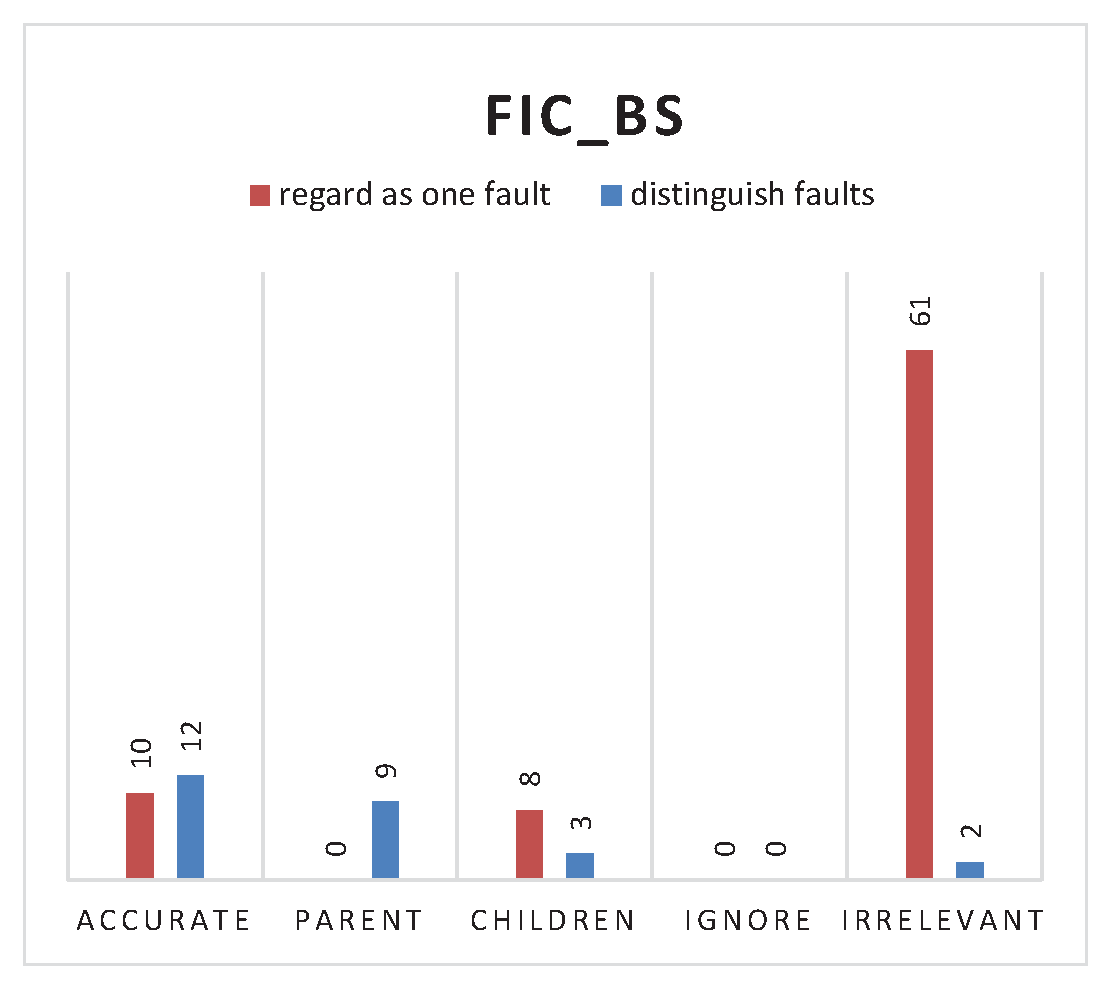
\includegraphics[width=2.21in]{FIC_BS_normal.eps}
}
\subfigure[]{
  %  \rule{4cm}{3cm}
    \label{fig:subfig2}
    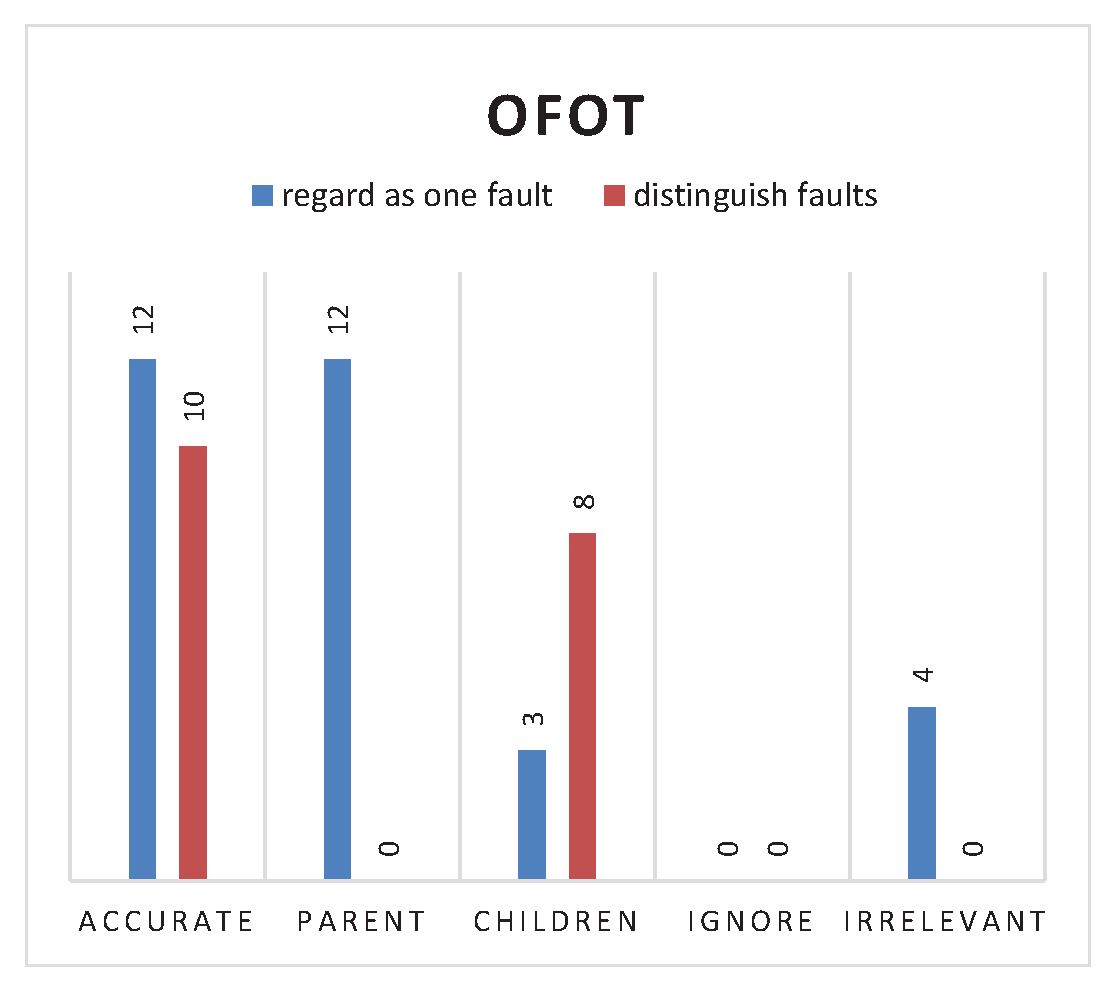
\includegraphics[width=2.21in]{OFOT_normal.eps}
}
\subfigure[]{
  %  \rule{4cm}{3cm}
    \label{fig:subfig3}
    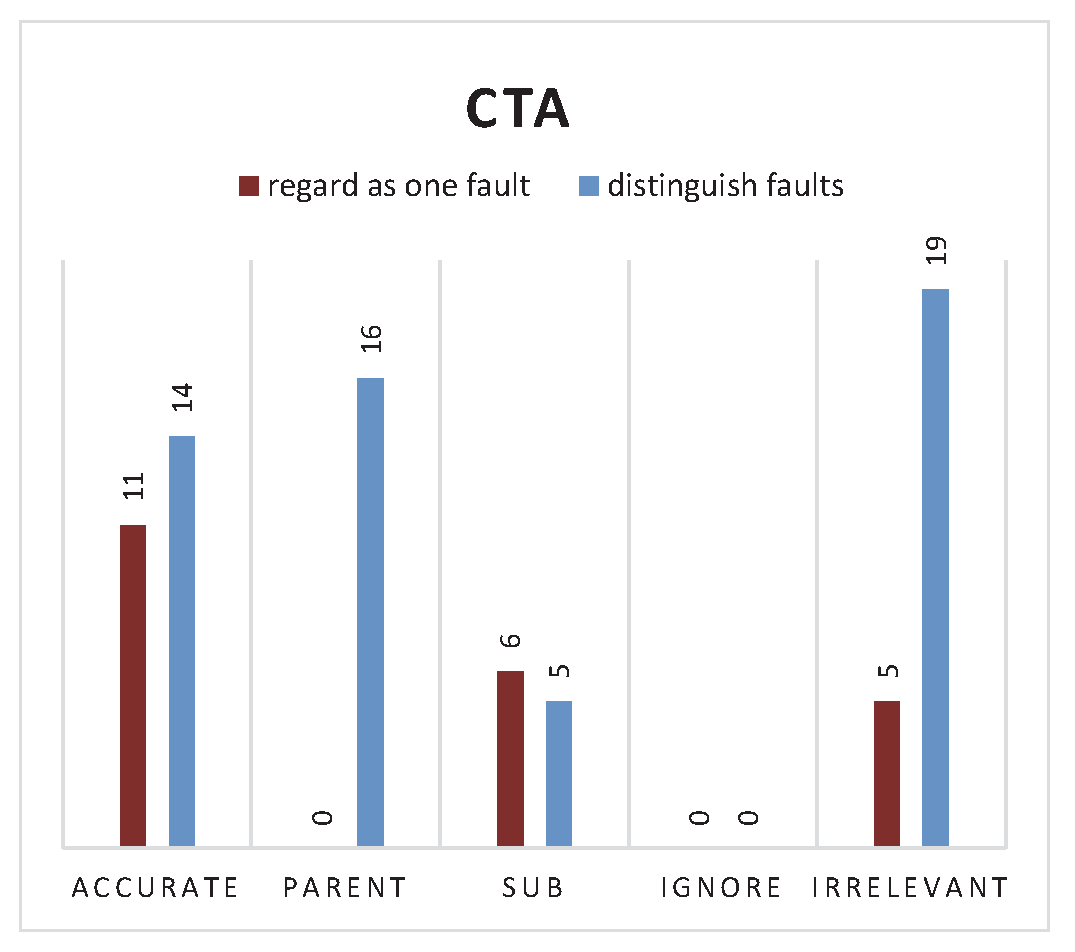
\includegraphics[width=2.21in]{CTA_normal.eps}
}
\caption[]{Results of two strategies for traditional approaches: FIC\_BS, OFOT and CTA}
\label{fig:normalexperiment}
\end{figure*}

We first observed that, traditional approaches do suffer from the masking effect to some extent. Specifically, in the Figure \ref{fig:subfig1}, FIC\_BS approach only correctly identified 12 and 10 accurate combinations for the two traditional strategies respectively, while wrongly identified 14 and 69 combinations, in which for the identified parent combinations, identified sub combinations, identified irreverent combinations are 9,3,2 and 0,8,61 respectively. This is similar to the result illustrated in Figure \ref{fig:subfig2} and \ref{fig:subfig3} for approach OFOT and CTA .

Another interesting observations is that for the \emph{regard as one fault} and \emph{distinguish faults} strategy, the former get more \emph{sub combinations} than later, while \emph{distinguish faults} strategy get more \emph{parent combinations} than \emph{regard as one}. This result accorded with our formal analysis in section 3.2. With respect to the metrics \emph{irrelevant combinations}, however, we didn't get as expected as in the formal analysis. In fact, both the case that \emph{regard as one fault} has more \emph{irrelevant combinations} ( see Figure \ref{fig:subfig1}) and the case that \emph{distinguish faults} has more (see Figure \ref{fig:subfig2} and \ref{fig:subfig3}) exist. With checking the executing process and the combinations they got, we believed one possible main reason for this result is that the algorithm encountered the problem of importing newly faults which bias their identifying process.

%\emph{regard as one fault} would get more \emph{} except the following case,  An exception is for the FIC\_BS, which we think when consider the regard as one fault faults strategy, it increase the possibility that import newly bugs so that bais the result. it always that . fahter and parent. which are accordant with the analysis in the formal model.

We further observed that, for different algorithms, the extent to what they suffered from masking effects varied. For instance, for FIC\_BS approach, under the masking effects, they  identified the 61 and 2 irrelevant combinations for two strategies, while for OFOT and CTA, this value is 0 and 4, 5 and 19 respectively. There are two factors caused this difference: the chosen test cases and the analysis method. For FIC\_BS and OFOT this two methods, the test cases they chosen for isolating failure-inducing combinations is different, which consequently changed the masking effects they may encountered. For OFOT an CTA, while the test cases we chosen is the same, the difference lies at the way they characterizing the failure-inducing combinations in the test cases, which OFOT directly identify the parameter in the passed test cases while CTA used classified tree analysis.

%
%From this figure, we can easily find that Traditional MFS identifying approaches do suffer from the multiple faults and their masking effect. For example, for the Grep, version 3.14, all these three algorithm will lost some information. Additionally, the extent to which the impact has affected vary from algorithms. We can find that for HSQLDB with version 3.14, the similarity of CTA was just at 4 while FIC is 3. We list these points in figure 3. From this figure, we can learn that.

Therefore, the answer we got for \textbf{Q2} is: traditional algorithm do suffer from the multiple faults and their masking effect, although the extent vary in different algorithms.

\subsection{Performance of our approach}
The last case study aims to observe the performance of our approach and compare it with the result got by the traditional approaches. Our approach augment the three traditional FCI approaches with replacing test cases strategy described in Section 4, and then we applied these augmented approaches to identify the failure-inducing combinations in the prepared subjects.

\subsubsection{Study setup}
The setup of this case study is almost the same as the second case study. The difference is that the algorithms we choose are three augment ones. Additionally, comparisons between augment approaches with three traditional ones will be quantified.

\subsubsection{Result and discussion}
Figure \ref{fig:subfigureExample2} presents the result of the last case study. The organization of this figure is similar to the second study. The bar in each column depicts the results the augment approaches, which labelled as "replacing strategy". We marked two additional points in each column which represent the result of \emph{regard as one fault} and \emph{distinguish faults} strategy to get a comparison with the augment approaches.

% We just added some information in the parentheses attached the value in each cell. This information display the  discrepancy between traditional ones. Notation '+' means promotions against traditional ones, while '-' indicates decrease. The value in parentheses has been normalized.

\begin{figure*}[ht]
\centering
\subfigure[]{
  %  \rule{4cm}{3cm}
    \label{fig:subfig4}
    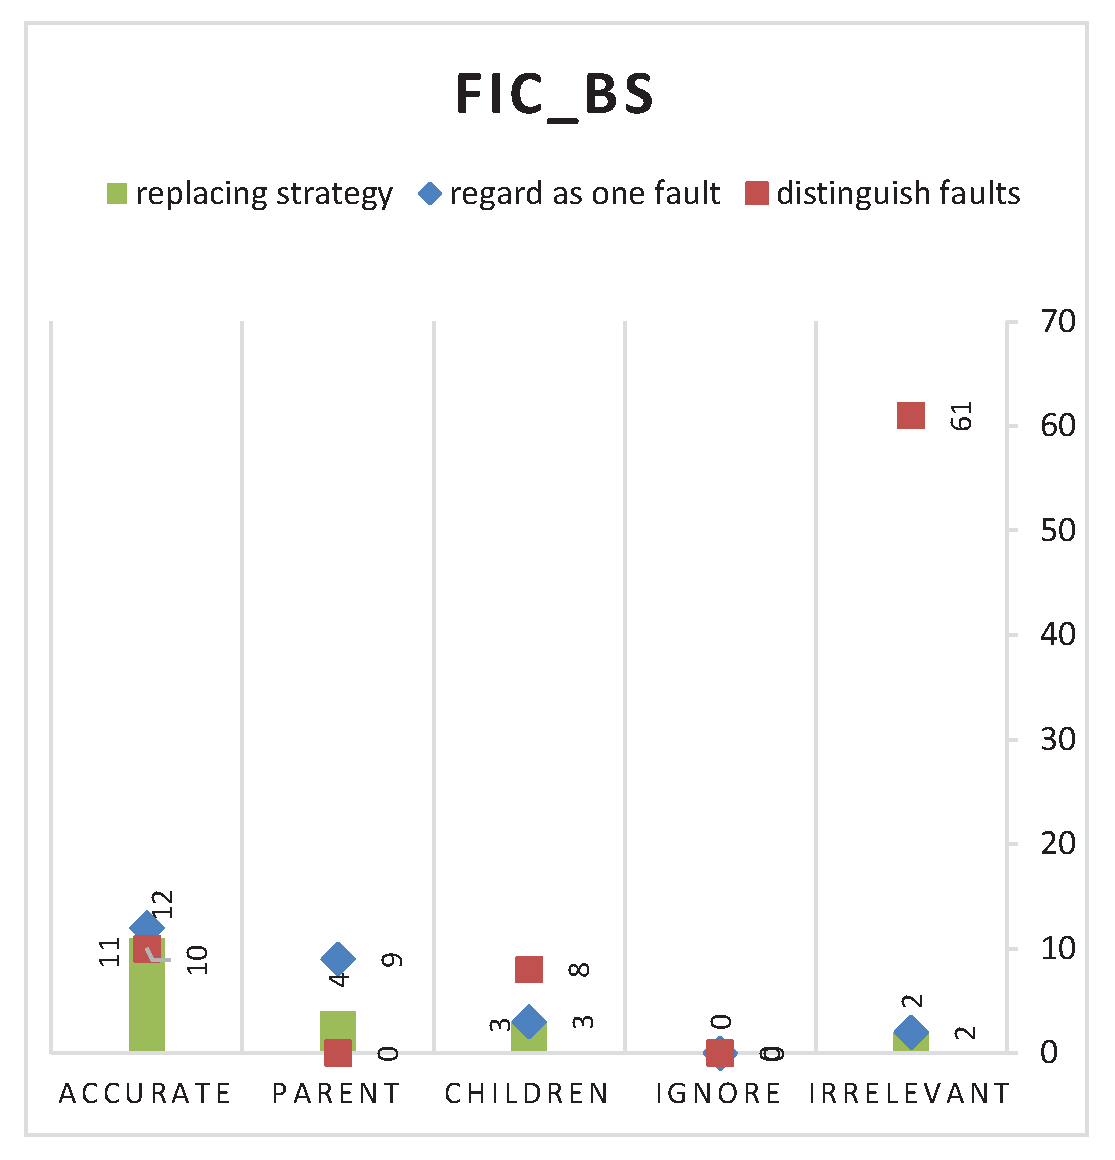
\includegraphics[width=2.21in]{FIC_BS_our.eps}
}
\subfigure[]{
  %  \rule{4cm}{3cm}
    \label{fig:subfig5}
    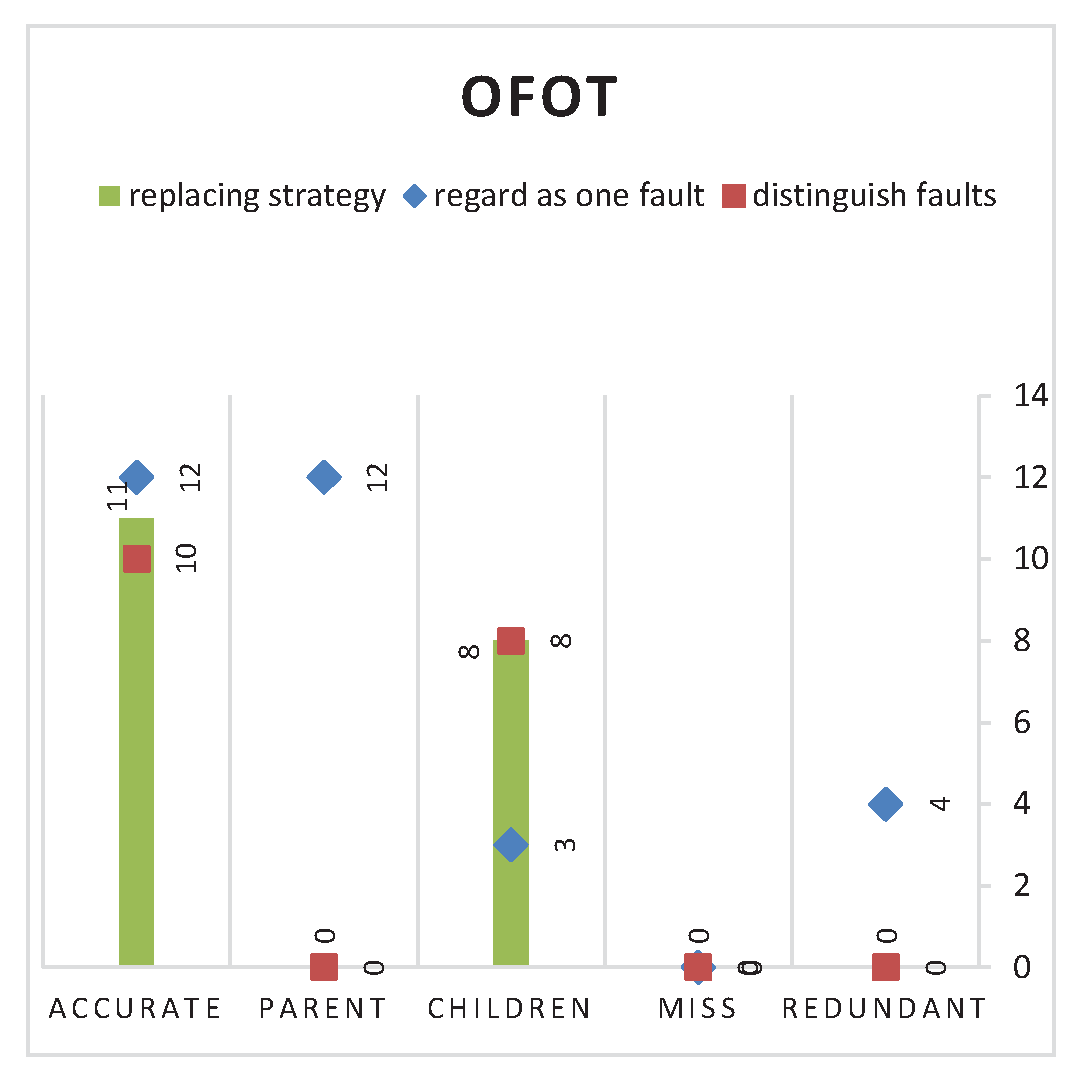
\includegraphics[width=2.21in]{OFOT_our.eps}
}
\subfigure[]{
  %  \rule{4cm}{3cm}
    \label{fig:subfig6}
    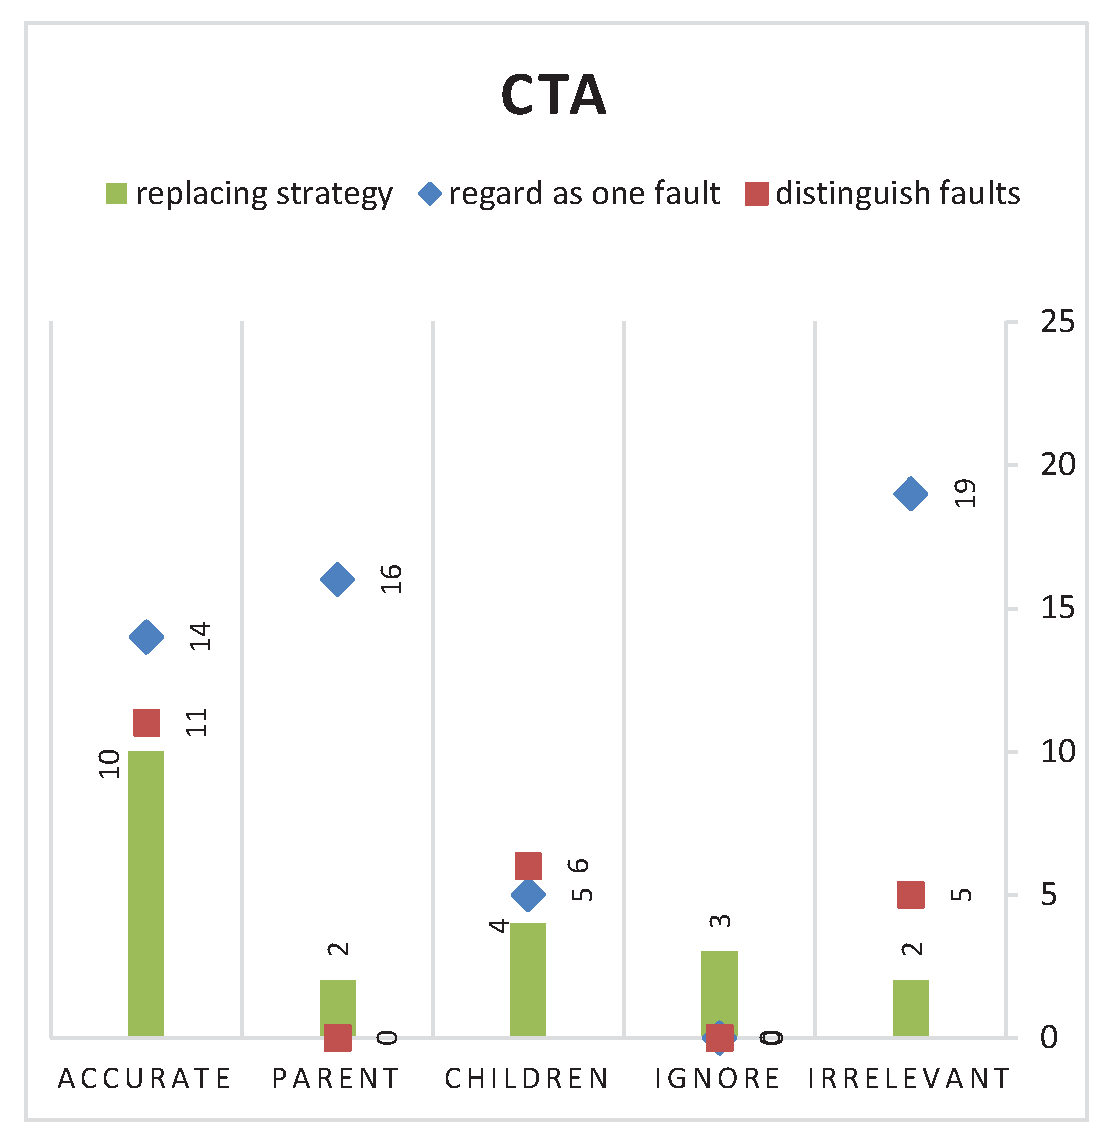
\includegraphics[width=2.21in]{CTA_our.eps}
}
\caption[Optional caption for list of figures]{Three approaches augmented with the replacing strategy}
\label{fig:subfigureExample2}
\end{figure*}


Comparing the augment approach with two traditional strategies in Figure \ref{fig:subfigureExample2}, we observed that there is significant improvement for augment approach in reducing the wrongly identified combinations. For instance, CTA approach in Figure \ref{fig:subfig6} only got 2 irrelevant combinations with replacing strategy, while the traditional two strategy get 5 and 19 irrelevant combinations respectively. And for FIC\_BS in Figure \ref{fig:subfig4} this comparison is 2 for replacing strategy, and 2 , 61 for two traditional strategies.

Besides, the augment approach also get a good performance at limiting the number of identified sub combinations and parent combination. In effect, compared with \emph{distinguish faults} which good at limiting sub combinations while producing more parent combinations and \emph{regard as one fault} which is the other way around, the augment ones get a more balanced result. Specifically, for instance, in Figure \ref{fig:subfig4} for approach FIC\_BS, \emph{distinguish faults} strategy got 9 parent combinations while got 3 sub combinations. And for \emph{regard as one fault} strategy, it got none parent combination but got 8 sub combinations. For the replacing strategy, it only get 4 parent combination, which smaller than \emph{distinguish faults} strategy, and get 3 sub combinations which smaller than regard as one fault strategy and equal to \emph{distinguish faults} strategy.

Apart from these improvement, there is some slight decline for the augment approach. We noted that for replacing strategy, it nearly got 2 less accurate combinations on average than traditional strategies, and ignored 1 more failure-inducing combinations on average than traditional ones.
% Further more it also that number of correctly identified combinations with replacing strategy slightly declines than traditional ones(about 2 less in average).

%As a compensation, however, We noted that the augment approaches got slightly . But promotions against traditional ones. In fact, there are 10 out of 14 cases that augment ones outperform traditional ones at the metric of "similarity", and 9 out of 14 cases that augment ones are better than traditional ones at the metric of "num diff". Additional, this promotion is distinct. As we can see, the best promotion for similarity is 0.9 and the best promotion for num diff is 0.7. Furthermore, the average performance promotion for similarity reached '+ 0.6' and this value reached '+ 0.5' for the num diff metric.

In summary, the answer for \textbf{Q3} is: our approach do get make the FCI approaches get better better performance at identifying failure-inducing combinations when facing masking effect between multiple faults to some extent.

\subsection{Threats to validity}
There are several threats to validity for these empirical studies. First, we have only surveyed five open-source software, four of which are medium-sized and one is large-sized. This may impact the generality of our observations. Although we believe it is quite possible a common phenomenon in most software that contain multiple faults which can mask each other, we need to investigate more software to support our conjecture.

The second threat comes from the input model we built. As we focused on the options related to the perfect combinations and only augmented it with some noise options, there is a chance we will get different result if we choose other noise options. More different options needed to be opted to see whether our result is common or just appeared in some particular input model.

The third threats is that we just observed three failure-inducing combinations identifying algorithms, further works needed to examine more algorithms in this filed to get a more general result.

\section{related works}

Shi in \cite{shi2005software} presented a further testing strategy for fault revealing and failure diagnosis, which first tests SUT with a covering array, then reduces the value schemas contained in the failed test case by eliminating those appearing in the passed test cases. If the failure-causing schema is found in the reduced schema set, failure diagnosis is completed with the identification of the specific input values which caused the failure;
otherwise, a further test suite based on SOFOT is developed for each failed test cases,
testing is repeated, and the schema set is then further reduced, until no more failure
is found or the fault has been located. Based on this work, Wang in \cite{wang2010adaptive} proposed an AIFL approach which extended the SOFOT process by mutating the changing strength in each iteration of characterizing failure-inducing combinations.

Nie's in \cite{nie2011minimal} introduced the notion of Minimal Failure-causing Schema(MFS) and proposed the OFOT approach which extended from SOFOT that can isolate the MFS in SUT. The approach mutants one value with different values for that parameter, hence generating a group of additional test cases each time to be executed. Compared with SOFOT, this approach  strengthen the validation of the factor under analysis and also can detect the newly imported faulty combinations.

Delta debugging \cite{zeller2002simplifying} proposed by Zeller is an adaptive divide-and-conquer approach to locate interaction fault. It is very efficient and has been applied to real software environment. Zhang et al. \cite{zhang2011characterizing} also proposed a similar approach that can identify the failure-inducing combinations that has no overlapped part efficiently. Later Li in \cite{li2012improved} improved the delta-debugging based failure-inducing combination by exploiting the useful information in the executed covering array.

Colbourn and McClary \cite{colbourn2008locating} proposed a non-adaptive method. Their approach extends the covering array to the locating array to detect and locate interaction faults. C. Martinez \cite{martinez2008algorithms,martinez2009locating} proposed two adaptive algorithms. The first one needs safe value as their assumption and the second one remove the assumption when the number of values of each parameter is equal to 2. Their algorithms focus on identifying the faulty tuples that have no more than 2 parameters.

Ghandehari.etc \cite{ghandehari2012identifying} defines the suspiciousness of tuple and suspiciousness of the environment of a tuple. Based on this, they rank the possible tuples and generate the test configurations. Although their approach imposes minimal assumption, it does not ensure that the tuples ranked in the top are the faulty tuples. They further in \cite{ghandehari2013fault} utilzed the test cases generated from the inducing combination to locate the faults inside the source code.


Yilmaz \cite{yilmaz2006covering} proposed a machine learning method to identify inducing combinations from a combinatorial testing set. They construct a classified tree to analyze the covering arrays and detect potential faulty combinations. Beside this, Fouché \cite{fouche2009incremental} and Shakya \cite{shakya2012isolating} made some improvements in identifying failure-inducing combinations based on Yilmaz's work.

Our previous work \cite{niu2013identifying} have proposed an approach that utilize the tuple relationship tree to isolate the failure-inducing combinations in a failing test case. One novelty of this approach is that it can identify the overlapped faulty combinations. This work also alleviates the problem of introducing newly failure-inducing combinations in additional test cases.

In addition to the works that aims at identifying the failure-inducing combinations in test cases, there are some studies focus on working around the masking effects:

With having known masking effects in prior, Cohen  in\cite{cohen2007exploiting,cohen2007interaction,cohen2008constructing} studied the impacts that the masking effects render some generated test cases invalid in CT, and they proposed the approach that integrate the incremental SAT solver with covering array generating algorithms to avoid these masking effects in test cases generating process. Further study was conducted in \cite{petke2013efficiency}to show the fact that with considering constrains, the higher-strength covering arrays with early fault detection is practical. Besides, additional constraints impacts in CT were studied in works like \cite{garvin2011evaluating,bryce2006prioritized,calvagna2008logic,grindal2006handling,yilmaz2013test}. %These approaches use some rules or to avoid these invalidated test cases to improve the efficiency when examine the test cases.

Chen etc. in \cite{chen2010combinatorial} addressed the issues of shielding parameters in combinatorial testing and proposed the Mixed Covering Array with Shielding Parameters (MCAS) to solve the problem caused by shielding parameters. The shielding parameters can disable some parameter values to expose additional interaction errors, which can be regarded as a special case of masking effects.

Dumlu and Ylimaz in \cite{dumlu2011feedback} proposed a feedback-driven approach to work around the masking effects. In specific, it first use CTA classify the possible failure-inducing combinations and then eliminate them and generate new test cases to detect possible masked interaction in the next iteration. They further extended their work in \cite{yilmaz2013reducing}, in which they proposed a multiple-class CTA approach to distinguish faults in SUT. In addition, they empirically studied the impacts on both ternary-class and multiple-class CTA approaches.

Our work differs from these ones mainly in the fact that we formally studied the masking effects on FCI approaches and further proposed a divide-and-conquer strategy to alleviate this impact.

\section{Conclusions}
Masking effects of multiple faults in SUT can bias the result of traditional failure-inducing combinations identifying approaches. In this paper, we formalized the process of identifying failure-inducing combinations under the circumstance that masking effects exist in SUT and try to understand how do this impacts brought by masking effect. Furthermore, we have presented a divide and conquer strategy to assist traditional FCI approaches to alleviate this impact.

%This strategy separately handle each fault in SUT, and for a particular fault, it will discard these test cases that trigger faults different from the one under analysis and only keep those that either pass or trigger the expected fault. Additional test cases for compensation will be generated after discarding unsatisfied test cases.

In the empirically studies, we extended three FCI approaches with our strategy. The comparison between this three traditional approaches and their variation is conducted on on several open-source software. The results shows that our strategy do assist traditional FCI approaches get a better performance when facing masking effects in SUT.

As a future work, we need to do more empirical studies to make our conclusion more general. Our current experimental subjects are several middle-sized software, we would like to extend our approach into more complicated and large-scaled testing scenarios. Another promising work in the future is to combine white-box testing technique to make the FCI approaches get more accurate results when handling masking effects. We believe that figuring out the fault levels of different bugs through white-box testing technique is helpful to reduce misjudgement in the failure-inducing combinations identifying process. As one important observation is that the extent to what the FCI suffers from masking effects varies in different algorithms, so the combination of different FCI approaches is desired in the future to further improve the performance for handling
such effects.

%\end{document}  % This is where a 'short' article might terminate

%ACKNOWLEDGMENTS are optional
%\section{Acknowledgments}
%This section is optional; it is a location for you
%to acknowledge grants, funding, editing assistance and
%what have you.  In the present case, for example, the
%authors would like to thank Gerald Murray of ACM for
%his help in codifying this \textit{Author's Guide}
%and the \textbf{.cls} and \textbf{.tex} files that it describes.

%
% The following two commands are all you need in the
% initial runs of your .tex file to
% produce the bibliography for the citations in your paper.
\bibliographystyle{abbrv}
%\bibliographystyle{unsrt}
\bibliography{sigproc}  % sigproc.bib is the name of the Bibliography in this case
% You must have a proper ".bib" file
%  and remember to run:
% latex bibtex latex latex
% to resolve all references
%
% ACM needs 'a single self-contained file'!
%
%APPENDICES are optional
%\balancecolumns
%\appendix
%%Appendix A
\end{document}
